\chapter{Interval-based system models: timelines}\label{chap:Timelines}
\begin{chapref}
The references for this chapter are~\cite{kr18,gand18,ictcs18}.
\end{chapref}

\minitoc\mtcskip

\newcommand{\Instruct}{\mathsf{Inst}}
\newcommand{\InstructLab}{\mathsf{InstLab}}
\newcommand{\InstL}{\mathsf{L}}
\newcommand{\Inc}{\mathsf{Inc}}
\newcommand{\Dec}{\mathsf{Dec}}
\newcommand{\halt}{{\textit{halt}}}
\newcommand{\init}{{\textit{init}}}
\newcommand{\main}{{\textit{main}}}
\newcommand{\Checking}{{\textit{check}}}
\newcommand{\inc}{{\mathsf{inc}}}
\newcommand{\dec}{{\mathsf{dec}}}

\newcommand{\zero}{{\mathsf{zero}}}
\newcommand{\instr}{{\textit{op}}}
\newcommand{\gainy}{{\textit{gainy}}}
\newcommand{\From}{{\textit{from}}}
\newcommand{\To}{{\textit{to}}}
\newcommand{\cont}{{\textit{sec}}}
\newcommand{\Tag}{{\textit{Tag}}}
\newcommand{\Succ}{{\textit{succ}}}
\newcommand{\op}{{\textit{op}}}

\newcommand{\dummy}{{\textit{dummy}}}

\newcommand{\Con}{\mathsf{con}}


\newcommand{\start}{\mathsf{s}}
\newcommand{\startTime}{\mathsf{s}}
\newcommand{\Ending}{\mathsf{e}}


\newcommand{\der}[1]{\ensuremath{\;\;{\mathop{{ %
            \longrightarrow}}\limits^{{#1}}}\!}\;\;} %

\newcommand{\derG}[1]{\ensuremath{\;\;{\mathop{{ %
            \longrightarrow}}\limits^{{#1}}}\!}_\gainy\;\;} %


%%%%%%%%%%%%%%%%%%%%%%%%%%%
\newcommand{\TA}{\text{\sffamily TA}}
\newcommand{\MTL}{\text{\sffamily MTL}}
\newcommand{\TPTL}{\text{\sffamily TPTL}}
\newcommand{\MITL}{\text{\sffamily MITL}}
\newcommand{\MITLR}{\text{\sffamily MITL}_{(0,\infty)}}

\newcommand{\RealP}{{\mathbb{R}_+}}
\newcommand{\RatP}{{\mathbb{Q}_+}}
\newcommand{\val}{{\mathit{val}}}
\newcommand{\Main}{{\mathit{Main}}}
\newcommand{\EqTime}{{\mathit{EqTime}}}
\newcommand{\Past}{{\mathit{past}}}
\newcommand{\code}{{\mathit{code}}}
\newcommand{\Res}{\textit{Res}}
\newcommand{\TLang}{{\mathcal{L}_T}}
\newcommand{\StrictUntil}{\textsf{U}}

%\newcommand{\DefORmini}{\ensuremath{\;\big|\;}}
\newcommand{\Deriv}{{\mathit{Deriv}}}
\newcommand{\Intv}{{\mathit{Intv}}}
\newcommand{\IntvR}{{\mathit{Intv}_{(0,\infty)}}}



%# -*- coding: utf-8-unix -*-
%%==================================================
%% chapter01.tex for SJTU Master Thesis
%%==================================================

%\bibliographystyle{sjtu2}%[此处用于每章都生产参考文献]
\chapter{这是什么}
\label{chap:intro}

这是上海交通大学(非官方)学位论文 \LaTeX 模板,当前版本是 \version 。

最早的一版学位模板是一位热心的物理系同学制作的。
那份模板参考了自动化所学位论文模板,使用了CASthesis.cls文档类,中文字符处理则采用当时最为流行的 \CJKLaTeX 方案。
我根据交大研究生院对学位论文的要求
\footnote{\url{http://www.gs.sjtu.edu.cn/policy/fileShow.ahtml?id=130}}
,结合少量个人审美喜好,完成了一份基本可用的交大 \LaTeX 学位论文模板。
但是,搭建一个 \CJKLaTeX 环境并不简单,单单在Linux下配置环境和添加中文字体,就足够让新手打退堂鼓。
在William Wang的建议下,我开始着手把模板向 \XeTeX 引擎移植。
他完成了最初的移植,多亏了他出色的工作,后续的改善工作也得以顺利进行。

随着我对 \LaTeX 系统认知增加,我又断断续续做了一些完善模板的工作,在原有硕士学位论文模板的基础上完成了交大学士和博士学位论文模板。

现在,交大学位论文模板SJTUTHesis代码在github
\footnote{\url{https://github.com/sjtug/SJTUThesis}}
上维护。
你可以\href{https://github.com/sjtug/SJTUThesis/issues}{在github上开issue}
、或者在\href{https://bbs.sjtu.edu.cn/bbsdoc?board=TeX_LaTeX}{水源LaTeX版}发帖来反映遇到的问题。

\section{使用模板}

\subsection{准备工作}
\label{sec:requirements}

要使用这个模板撰写学位论文,需要在\emph{TeX系统}、\emph{TeX技能}上有所准备。

\begin{itemize}[noitemsep,topsep=0pt,parsep=0pt,partopsep=0pt]
	\item {\TeX}系统:所使用的{\TeX}系统要支持 \XeTeX 引擎,且带有ctex 2.x宏包,以2015年的\emph{完整}TeXLive、MacTeX发行版为佳。
	\item TeX技能:尽管提供了对模板的必要说明,但这不是一份“ \LaTeX 入门文档”。在使用前请先通读其他入门文档。
	\item 针对Windows用户的额外需求:学位论文模本分别使用git和GNUMake进行版本控制和构建,建议从Cygwin\footnote{\url{http://cygwin.com}}安装这两个工具。
\end{itemize}

\subsection{模板选项}
\label{sec:thesisoption}

sjtuthesis提供了一些常用选项,在thesis.tex在导入sjtuthesis模板类时,可以组合使用。
这些选项包括:

\begin{itemize}[noitemsep,topsep=0pt,parsep=0pt,partopsep=0pt]
	\item 学位类型:bachelor(学位)、master(硕士)、doctor(博士),是必选项。
	\item 中文字体:fandol(Fandol 开源字体)、windows(Windows 系统下的中文字体)、mac(macOS 系统下的华文字体)、ubuntu(Ubuntu 系统下的文泉驿和文鼎字体)、adobe(Adobe 公司的中文字体)、founder(方正公司的中文字体),默认根据操作系统自动配置。
	\item 英文模版:使用english选项启用英文模版。
	\item 盲审选项:使用review选项后,论文作者、学号、导师姓名、致谢、发表论文和参与项目将被隐去。
\end{itemize}

\subsection{编译模板}
\label{sec:process}

模板默认使用GNUMake构建,GNUMake将调用latemk工具自动完成模板多轮编译:

\begin{lstlisting}[basicstyle=\small\ttfamily, caption={编译模板}, numbers=none]
make clean thesis.pdf
\end{lstlisting}

若需要生成包含“原创性声明扫描件”的学位论文文档,请将扫描件保存为statement.pdf,然后调用make生成submit.pdf。

\begin{lstlisting}[basicstyle=\small\ttfamily, caption={生成用于提交的学位论文}, numbers=none]
make clean submit.pdf
\end{lstlisting}

编译失败时,可以尝试手动逐次编译,定位故障。

\begin{lstlisting}[basicstyle=\small\ttfamily, caption={手动逐次编译}, numbers=none]
xelatex -no-pdf thesis
biber --debug thesis
xelatex thesis
xelatex thesis
\end{lstlisting}

\subsection{模板文件布局}
\label{sec:layout}

\begin{lstlisting}[basicstyle=\small\ttfamily,caption={模板文件布局},label=layout,float,numbers=none]
├── LICENSE
├── Makefile
├── README.md
├── bib
│   ├── chap1.bib
│   └── chap2.bib
├── bst
│   └── GBT7714-2005NLang.bst
├── figure
│   ├── chap2
│   │   ├── sjtulogo.eps
│   │   ├── sjtulogo.jpg
│   │   ├── sjtulogo.pdf
│   │   └── sjtulogo.png
│   └── sjtubanner.png
├── sjtuthesis.cfg
├── sjtuthesis.cls
├── statement.pdf
├── submit.pdf
├── tex
│   ├── abstract.tex
│   ├── ack.tex
│   ├── app_cjk.tex
│   ├── app_eq.tex
│   ├── app_log.tex
│   ├── chapter01.tex
│   ├── chapter02.tex
│   ├── chapter03.tex
│   ├── conclusion.tex
│   ├── id.tex
│   ├── patents.tex
│   ├── projects.tex
│   ├── pub.tex
│   └── symbol.tex
└── thesis.tex
\end{lstlisting}

本节介绍学位论文模板中木要文件和目录的功能。

\subsubsection{格式控制文件}
\label{sec:format}

格式控制文件控制着论文的表现形式,包括以下几个文件:
sjtuthesis.cfg, sjtuthesis.cls和GBT7714-2005NLang.bst。
其中,“cfg”和“cls”控制论文主体格式,“bst”控制参考文献条目的格式,

\subsubsection{主控文件thesis.tex}
\label{sec:thesistex}

主控文件thesis.tex的作用就是将你分散在多个文件中的内容“整合”成一篇完整的论文。
使用这个模板撰写学位论文时,你的学位论文内容和素材会被“拆散”到各个文件中:
譬如各章正文、各个附录、各章参考文献等等。
在thesis.tex中通过“include”命令将论文的各个部分包含进来,从而形成一篇结构完成的论文。
对模板定制时引入的宏包,建议放在导言区。

\subsubsection{各章源文件tex}
\label{sec:thesisbody}

这一部分是论文的主体,是以“章”为单位划分的,包括:

\begin{itemize}[noitemsep,topsep=0pt,parsep=0pt,partopsep=0pt]
	\item 中英文摘要(abstract.tex)。前言(frontmatter)的其他部分,中英文封面、原创性声明、授权信息在sjtuthesis.cls中定义,不单独分离为tex文件。
不单独弄成文件。
	\item 正文(mainmatter)——学位论文正文的各章内容,源文件是chapter\emph{xxx}.tex。
	\item 附录(app\emph{xx}.tex)、致谢(thuanks.tex)、攻读学位论文期间发表的学术论文目录(pub.tex)、个人简历(resume.tex)组成正文后的部分(backmatter)。
参考文献列表由bibtex插入,不作为一个单独的文件。
\end{itemize}

\subsubsection{图片文件夹figure}
\label{sec:fig}

figure文件夹放置了需要插入文档中的图片文件(支持PNG/JPG/PDF/EPS格式的图片),可以在按照章节划分子目录。
模板文件中使用\verb|\graphicspath|命令定义了图片存储的顶层目录,在插入图片时,顶层目录名“figure”可省略。

\subsubsection{参考文献数据库bib}
\label{sec:bib}

目前参考文件数据库目录只存放一个参考文件数据库thesis.bib。
关于参考文献引用,可参考第\ref{chap:example}章中的例子。


\section{The TP Problem}\label{sec:preliminTimelines}

As in the previous chapters, let $\Nat$ be the set of natural numbers and $\RealP$ be the set of non-negative real numbers; moreover, $\Intv$ denotes the set of intervals of $\RealP$ whose endpoints are in $\Nat\cup\{\infty\}$, and $\Intv_{(0,\infty)}$ is the set of non-singular%
\footnote{An interval of the form $[a,a]$, for $a\in\Nat$, is called \emph{singular}.} 
intervals $I\in \Intv$ such that
  either $I$ is unbounded, or $I$
  is left-closed with left endpoint $0$. The latter intervals $I$ can be replaced by expressions of the form $\sim n$, for some $n\in\Nat$
  and $\sim\,\in\{<,\leq,>,\geq\}$.
%
% Let $w$ be a finite word over some alphabet. By $|w|$ we denote the length of $w$. For all  $0\leq i<|w|$,  $w(i)$ is
% the $i$-th letter of $w$.


%\subsection{}\label{sec:timelines}

We now introduce notation and basic notions of
the TP framework as presented in~\cite{MayerOU16,GiganteMCO16}.
%
In TP, domain knowledge is encoded by a set of state variables, whose behaviour over time is described by transition functions and synchronization rules.

\begin{definition}[State variable]
  \label{def:statevar}
  A \emph{state variable} $x$ is a triple \[x= (V_x,T_x,D_x),\] where 
  \begin{itemize}
      \item $V_x$ is the \emph{finite domain} of the state variable $x$,
      \item $T_x:V_x\to 2^{V_x}$ is the \emph{value transition function}, which maps
        each $v\in V_x$ to the (possibly empty) set of successor values, and
      \item $D_x:V_x\to \Intv$ is the \emph{constraint (or duration) function} that maps each $v\in V_x$
        to an interval of $\Intv$.
  \end{itemize}   
\end{definition}

A \emph{token} for a variable $x$ is a pair $(v,d)$ consisting of a value $v\in V_x$ and a duration $d\in \RealP$
such that $d\in D_x(v)$. Intuitively, a token for $x$ represents an interval of time where the state variable $x$ takes value $v$.
In order to clarify the variable to which a token refers, we shall often denote $(v,d)$ as $(x,v,d)$.

The behavior of the state variable $x$ is specified by means of a \emph{timeline}, which is a non-empty sequence of tokens
$\pi = (v_0,d_0)\cdots  (v_n,d_n)$  consistent with the value transition function $T_x$, namely, such that
$v_{i+1}\in T_x(v_i)$ for all $0\leq i<n$. The \emph{start time} $\start(\pi,i)$ and the \emph{end time} $\Ending(\pi,i)$ of the $i$-th token of the timeline
$\pi$  are defined respectively as follows: 
\[\start(\pi,i)=0 \text{ if } i=0, \qquad \start(\pi,i)=\sum_{h=0}^{i-1} d_h \text{ otherwise},\]
and
\[\Ending(\pi,i)=\sum_{h=0}^{i} d_h.\]
%
See Figure~\ref{fig:timelineEx} for an example.
\begin{figure}
    \centering
    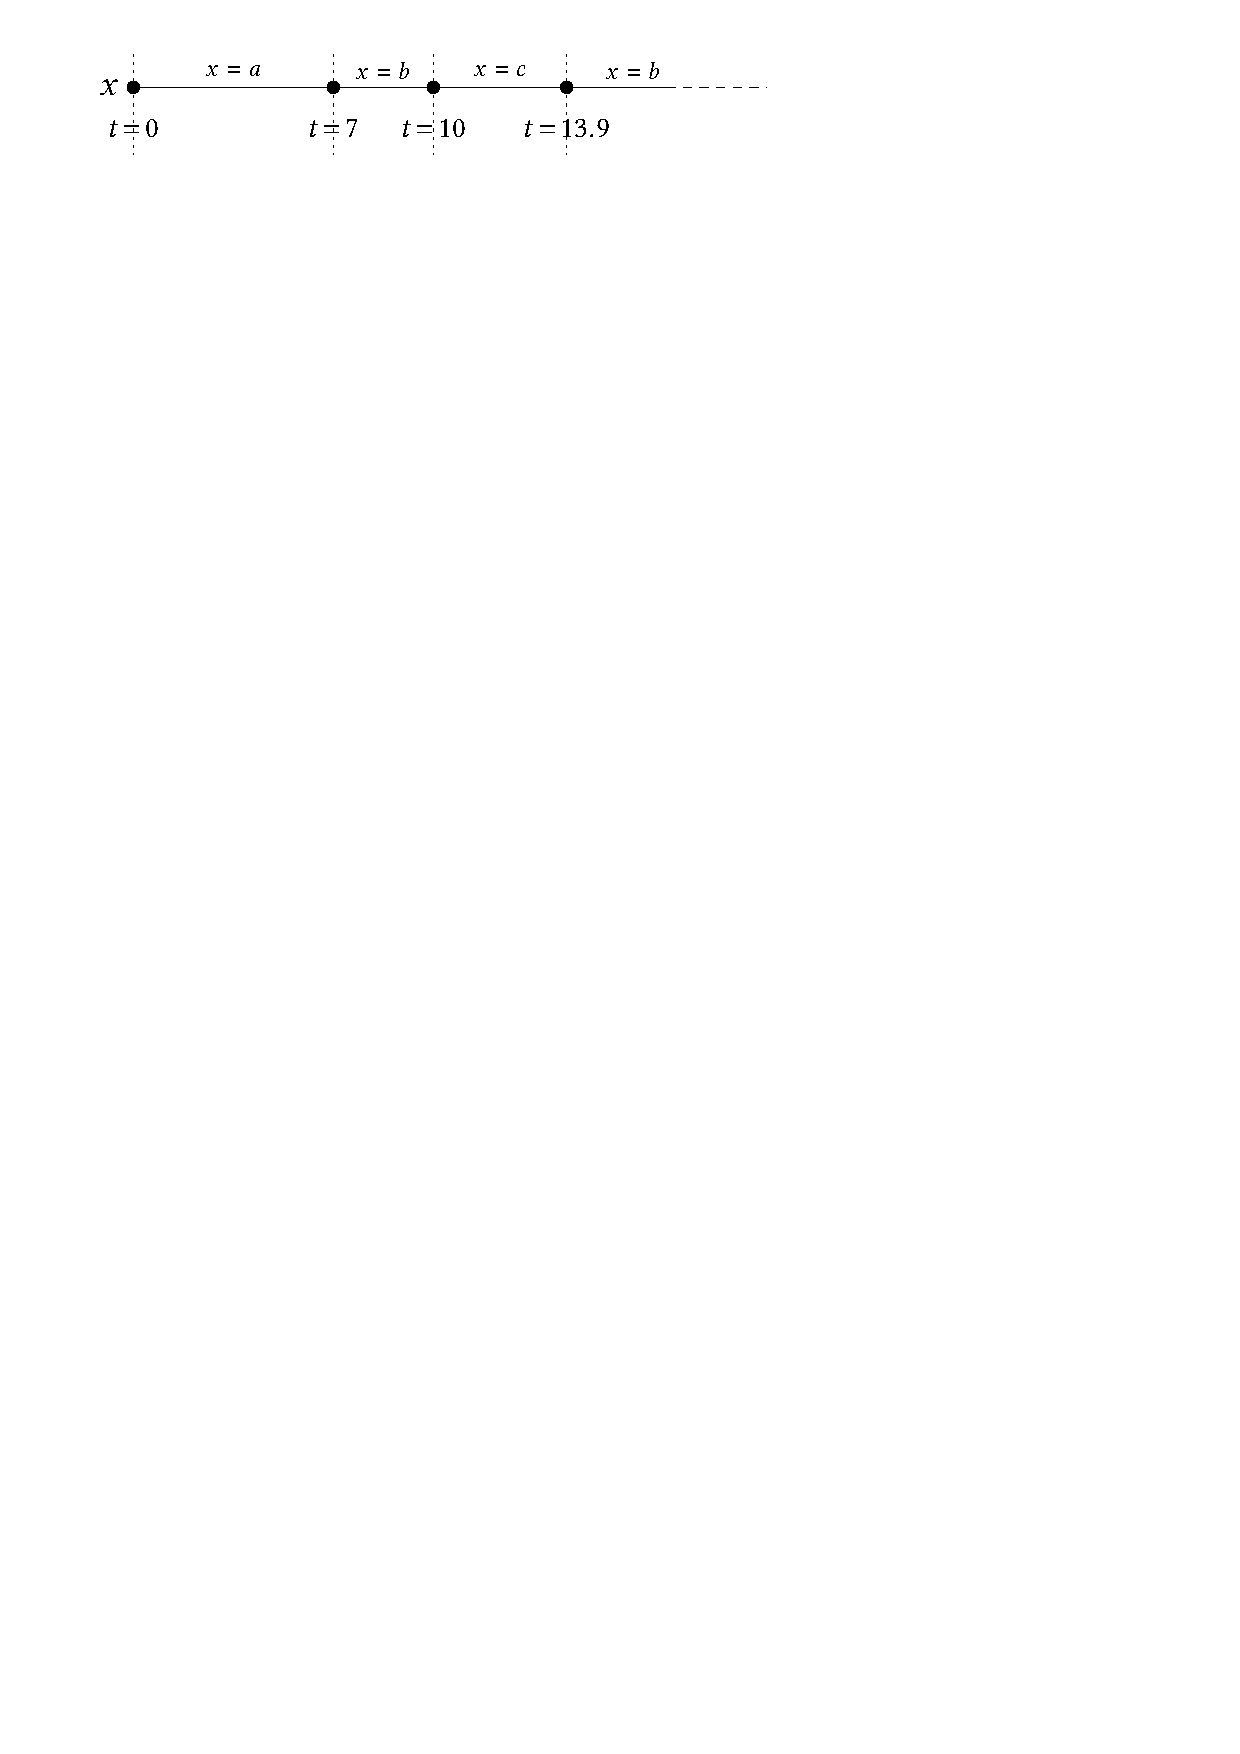
\includegraphics[scale=0.7]{Chaps/Timelines/timelineFig0.pdf}
    \caption{An example of timeline $(a,7)(b,3)(c,3.9)\cdots$ for the state variable $x= (V_x,T_x,D_x)$, where $V_x=\{a,b,c,\ldots\}$, $b\in T_x(a)$, $c\in T_x(b)$, $b\in T_x(c)$\dots\ and $D_x(a)=[5,8]$, $D_x(b)=[1,4]$, $D_x(c)=[2,\infty[$\dots}
    \label{fig:timelineEx}
\end{figure}

Given a finite set $SV$ of state variables, a \emph{multi-timeline} of $SV$ is a mapping $\Pi$ assigning to
each state variable $x\in SV$ a timeline for $x$.

Multi-timelines of $SV$ can be constrained by a set of \emph{synchronization
rules}, which relate tokens, possibly belonging to different timelines, through
temporal constraints on the start/end times of tokens (time-point constraints) and on the difference
between start/end times of tokens (interval constraints). The synchronization rules exploit
an alphabet $\Sigma=\{o,o_0,o_1,o_2,\ldots\}$ of token names to refer to the tokens along a multi-timeline, and are based on the notions of
\emph{atom} and \emph{existential statement}.

\begin{definition}[Atom]
  \label{def:timelines:atom}
  An \emph{atom} $\rho$ is either a clause of the form \mbox{$o_1\leq^{e_1,e_2}_{I} o_2$}
  (\emph{interval atom}), or of the forms $o_1\leq^{e_1}_{I} n$ or  $n\leq^{e_1}_{I}
  o_1$ (\emph{time-point atom}), where $o_1,o_2\in\Sigma$, $I\in\Intv$, $n\in\Nat$, and $e_1,e_2\in\{\start,\Ending\}$.
\end{definition}

An atom $\rho$ is evaluated with respect to a \emph{$\Sigma$-assignment $\lambda_\Pi$} for a given multi-timeline $\Pi$,
which is a mapping assigning to each token name $o\in \Sigma$ a pair $\lambda_\Pi(o)=(\pi,i)$ such that $\pi$ is a timeline of $\Pi$ and $0\leq i<|\pi|$ is a position along $\pi$ (intuitively,
$(\pi,i)$ represents the token of $\Pi$ referenced by the name $o$).

An interval atom $o_1\leq^{e_1,e_2}_{I} o_2$  \emph{is satisfied by  $\lambda_\Pi$} if $e_2(\lambda_\Pi(o_2))-e_1(\lambda_\Pi(o_1))\in I$.
A point atom $o\leq^{e}_{I} n$  (respectively, $n\leq^{e}_{I}o$)   \emph{is satisfied by  $\lambda_\Pi$} if $n-e(\lambda_\Pi(o))\in I$ (respectively, $e(\lambda_\Pi(o))-n\in I$).

\begin{definition}[Existential statement]
 An \emph{existential statement} $\mathcal{E}$ for a finite set $SV$ of state variables is a statement of the form
\[
\mathcal{E}=  \exists o_1[x_1=v_1]\cdots \exists o_n[x_n=v_n].\mathcal{C},
\]
  where $\mathcal{C}$ %$\mathcal{C}=\rho_0\land\ldots\land\rho_m$
  is a conjunction of atoms,
  $o_i\!\in\!\Sigma$, $x_i\!\in\! SV$, $v_i\!\in\! V_{x_i}$, for
  $1\leq i\leq n$. 

The elements $o_i[x_i=v_i]$ are called
  \emph{quantifiers}. A token name used in $\mathcal{C}$, but not occurring in any
  quantifier, is said to be \emph{free}. 
\end{definition}

  Given a $\Sigma$-assignment $\lambda_\Pi$ for a multi-timeline $\Pi$ of $SV$,
  we say that \emph{$\lambda_\Pi$ is consistent with the existential statement $\mathcal{E}$} if, for each quantifier $o_i[x_i=v_i]$, we have
   $\lambda_\Pi(o_i)=(\pi,h)$, where $\pi=\Pi(x_i)$ and the $h$-th token of $\pi$ has value $v_i$. A multi-timeline $\Pi$ of $SV$ \emph{satisfies} $\mathcal{E}$
   if there exists a $\Sigma$-assignment $\lambda_\Pi$ for $\Pi$ consistent with $\mathcal{E}$ such that each atom in $\mathcal{C}$ is satisfied by
   $\lambda_\Pi$.

We can now introduce synchronization rules, which constrain tokens, possibly belonging to different timelines.
\begin{definition}[Synchronization rule]
  A \emph{synchronization rule} $\mathcal{R}$ for a finite set $SV$ of state variables is a rule of one of the forms
  \[
  o_0[x_0=v_0] \to \mathcal{E}_1\lor \mathcal{E}_2\lor \ldots \lor \mathcal{E}_k, \qquad
          \true \to \mathcal{E}_1\lor \mathcal{E}_2\lor \ldots \lor \mathcal{E}_k,
  \]
  where $o_0\in\Sigma$, $x_0\in SV$, $v_0\in V_{x_0}$, and $\mathcal{E}_1, \ldots, \mathcal{E}_k$
  are \emph{existential statements}. % where only $o_0$ may appear free.
  In rules of the first
  form (which are called \emph{trigger rules}), the quantifier $o_0[x_0=v_0]$ is called \emph{trigger}; we require that only $o_0$ may appear free in $\mathcal{E}_i$, for all $1\leq i\leq n$. In rules of the second form (\emph{trigger-less rules}), we require
  that no token name appears free.
  \newline
  A trigger rule $\mathcal{R}$ is \emph{simple} if, for each existential statement $\mathcal{E}$ of $\mathcal{R}$ and each token name $o$ distinct from the trigger, there is at most one \emph{interval atom}
  of $\mathcal{E}$ where $o$ occurs.
\end{definition}

Intuitively, the  trigger $o_0[x_0=v_0]$ acts as a universal quantifier, which
states that \emph{for all} the tokens of the timeline for
$x_0$, where $x_0$ takes the
value $v_0$, at least one of the existential statements $\mathcal{E}_i$ must be satisfied. 
As an example, \[o_0[x_0=v_0]\to \exists o_1[x_1=v_1].o_0\leq^{\mathsf{e},\mathsf{s}}_{[2,\infty[} o_1\] states that after \emph{every} token for $x_0$ with value $v_0$ there exists a token for $x_1$ with value $v_1$ \emph{starting} at least 2 time instants after the \emph{end} of the former.
Trigger-less rules simply assert the
satisfaction of some existential statement. The intuitive meaning of \emph{simple} trigger rules is that they disallow simultaneous comparisons of multiple time-events
 (start/end times of tokens) with a non-trigger reference time-event. 
 
 The semantics of synchronization rules is formally defined as follows.
\begin{definition}[Semantics of synchronization rules]\label{def:semanticsRules}
Let $\Pi$ be a multi-timeline of a set $SV$ of state variables.

Given a \emph{trigger-less rule} $\mathcal{R}$ of $SV$, \emph{$\Pi$ satisfies $\mathcal{R}$} if $\Pi$ satisfies some existential statement of $\mathcal{R}$.

Given a \emph{trigger rule} $\mathcal{R}$ of $SV$ with trigger $o_0[x_0=v_0]$, \emph{$\Pi$ satisfies   $\mathcal{R}$} if, for every position $i$ of the
 timeline $\pi=\Pi(x_0)$ for $x_0$ such that $\pi(i)=(v_0,d)$, there exists an existential statement $\mathcal{E}$ of $\mathcal{R}$  and a $\Sigma$-assignment
 $\lambda_\Pi$ for $\Pi$ consistent with $\mathcal{E}$ such that $\lambda_\Pi(o_0)= (\pi,i)$ and $\lambda_\Pi$ satisfies all the atoms of $\mathcal{E}$.
\end{definition}

In the paper, we shall also focus on a stronger notion of satisfaction of trigger rules, called \emph{satisfaction under the future semantics}: it requires that all non-trigger tokens selected by some quantifier
%in the selected existential statements compared with the trigger token
do not start \emph{strictly before} the start time of the trigger token.

\begin{definition}[Future semantics of trigger rules]\label{def:futurerules}
  A multi-timeline $\Pi$ of $SV$ satisfies a trigger rule \[\mathcal{R}= o_0[x_0=v_0] \to \mathcal{E}_1\vee \mathcal{E}_2\vee
  \ldots \vee \mathcal{E}_k\]   \emph{under the future semantics} if $\Pi$ satisfies the trigger rule obtained from
  $\mathcal{R}$ by replacing each existential statement \[\mathcal{E}_i=\exists o_1[x_1=v_1]\cdots \exists o_n[x_n=v_n].\mathcal{C}\]
  by \[\mathcal{E}_i'=\exists o_1[x_1=v_1]\cdots \exists o_n[x_n=v_n].\Big(\mathcal{C}\wedge  \bigwedge_{i=1}^{n} o_0\leq^{\start,\start}_{[0,+\infty[} o_i\Big).\]
\end{definition}

A \emph{TP domain} $P=(SV,R)$ is specified by a finite set $SV$ of state variables and
a finite set $R$ of synchronization rules for $SV$ modeling their admissible behaviors.
Trigger-less rules can be used to express initial, as well as intermediate conditions
and the goals of the problem, while trigger rules are much more powerful and useful, for instance, to specify invariants and response requirements. 

A \emph{plan for $P=(SV,R)$} is a  multi-timeline of $SV$ satisfying all the rules in $R$. A \emph{future plan for $P$} is defined in a similar way, but we require satisfaction under the future semantics of \emph{all} trigger rules.

In the next sections we will study the following decision problems:
\begin{description}
  \item[TP problem] Given a TP domain $P=(SV,R)$, is there a plan for $P$?
  \item[Future TP problem] Given a TP domain $P\!=\!(SV\!,R)$, is there a \emph{future} plan for $P$?
\end{description}
%
%\begin{definition}%[Planning problem]
%  \label{def:timelines:problem}
%  A timeline-based planning \emph{problem} is a pair $P=(SV,S)$, where $SV$ is
%  a set of state variables and $S$ is a set of synchronization rules involving
%  variables in $SV$.
%  A \emph{plan} for
%  $P$ is a set of timelines $\Pi$, one for each $x_i\in SV$, such
%  that all the synchronization rules in $S$ are satisfied by the set $\Gamma$
%  of all tokens involved in (any of) the timelines of $\Pi$.
%\end{definition}

Table~\ref{tab:complex} summarizes all the decidability and complexity results described in the following about the mentioned problems:
we will consider mixes of restrictions on TP involving trigger rules with future semantics, simple trigger rules, and intervals in atoms (of trigger rules) which are non-singular or in $\Intv_{(0,\infty)}$.

\begin{table}[t]
    \centering    
    \caption{Decidability and complexity of restrictions of the TP problem.}
    \label{tab:complex}
    \resizebox{\linewidth}{!}{
    \begin{tabular}{r|c|c}
    	%\hline 
    	& TP problem & Future TP problem \\ 
    	\hline 
    	Unrestricted & Undecidable & (Decidable?) Non-primitive recursive-hard \\ 
    	\hline 
    	Simple trigger rules & Undecidable & Decidable (non-primitive recursive) \\ 
    	\hline 
    	Simple trigger rules, & \multirow{2}{*}{?} & \multirow{2}{*}{$\EXPSPACE$-complete} \\ 
    	non-singular intervals & & \\
    	\hline 
    	Simple trigger rules, & \multirow{2}{*}{?} & \multirow{2}{*}{$\Psp$-complete} \\ 
    	intervals in $\Intv_{(0,\infty)}$ & & \\
    	\hline 
    	Trigger-less rules only & $\NP$-complete & // \\ 
    	%\hline 
    \end{tabular} 
    }
\end{table}

\section{TP over dense temporal domains is an undecidable problem}\label{sec:undecidability}

In this section, we
start by settling an important negative result, namely, we
show that the TP problem, in its full generality, is undecidable over dense temporal domains, even when a single state variable is involved.
Undecidability is proved via a reduction from the halting problem for \emph{Minsky $2$-counter machines}~\cite{Minsky67}. The proof somehow resembles the one for the satisfiability problem of Metric Temporal Logic (which will be formally introduced later, in Section~\ref{sec:DecisionProcedures}) with both past and future temporal modalities, interpreted on dense time~\cite{AlurH93}.

As a preliminary step, we give a short account of Minsky 2-counter machines. A Minsky 2-counter machine (or just \emph{counter machine} for short) is a tuple $M = \tpl{\Instruct,\ell_\init,\ell_\halt}$ consisting of a finite set $\Instruct$ of labeled instructions $\ell: \imath$, where $\ell$ is a label  and $\imath$ is an instruction for either
\begin{itemize}
  \item \emph{increment} of counter $h$: $c_h:= c_h+1$; \texttt{goto} $\ell_r$, or
  \item  \emph{decrement} of counter $h$: \texttt{if} $c_h\!>\!0$ \texttt{then} $c_h:= c_h-1$; \texttt{goto} $\ell_s$ \texttt{else goto} $\ell_t$,
\end{itemize}
where $h \in \{1, 2\}$,  $\ell_s\neq \ell_t$, and $\ell_r$ (respectively, $\ell_s, \ell_t$) is either a label of an instruction in $\Instruct$ or the halting label $\ell_\halt$. Moreover, $\ell_\init\in\Instruct$ is the label of a designated (\lq\lq initial\rq\rq) instruction.

An \emph{$M$-configuration} is a triple of the form $C=(\ell, n_1, n_2)$, where $\ell$ is the label of an instruction (intuitively, which is the one to be executed next), and $n_1,n_2\in\Nat$ are the current values of the two counters $c_1$ and $c_2$, respectively. 

$M$ induces a transition relation, denoted by $\stackrel{M}{\longrightarrow}$, over pairs of $M$-configurations: 
\begin{itemize}
    \item for an instruction with label $\ell$ incrementing $c_1$, we have $(\ell, n_1, n_2)\stackrel{M}{\longrightarrow} (\ell_r, n_1+1, n_2)$, and
    \item for an instruction decrementing $c_1$, we have $(\ell, n_1, n_2)\stackrel{M}{\longrightarrow} (\ell_s, n_1-1, n_2)$ if $n_1>0$, and $(\ell, 0, n_2)\stackrel{M}{\longrightarrow} (\ell_t, 0, n_2)$ otherwise. 
\end{itemize}
The analogous for instructions changing the value of $c_2$.

An \emph{$M$-computation} is a \emph{finite} sequence $C_1,\ldots ,C_k$ of $M$-configurations such that $C_i \stackrel{M}{\longrightarrow} C_{i+1}$ for all $1\leq i<k$.
%
$M$ \emph{halts} if there exists an $M$-computation starting at $(\ell_\init, 0, 0)$ and leading to 
$(\ell_{\halt}, n_1, n_2)$, for some $n_1,n_2\in\Nat$. 
Given a counter machine $M$,
the \emph{halting problem for $M$} is to decide whether $M$ halts, and it was proved to be \emph{undecidable} by Minsky~\cite{Minsky67}.

The rest of the section is devoted to showing the following result.
\begin{theorem}\label{theorem:undecidability}
The TP problem over dense temporal domains is undecidable (even when a single state variable is involved).
\end{theorem}
\begin{proof}
We prove the thesis by a reduction from the halting problem for Minsky $2$-counter machines. 
%
Let us introduce the following notational conventions:
\begin{itemize}
  \item for increment instructions $\ell : c_h:= c_h+1$; \texttt{goto} $\ell_r$, we define $c(\ell)= c_h$ and $\Succ(\ell)= \ell_r$;
  \item  for decrement instructions $\ell:$ \texttt{if} $c_h>0$ \texttt{then} $c_h:= c_h-1$; \texttt{goto}  $\ell_r$ \texttt{else goto} $\ell_s$,
  we define $c(\ell)= c_h$, $\dec(\ell)= \ell_r$, and $\zero(\ell)= \ell_s$.
\end{itemize}
Moreover, let $\InstructLab$ be the set of instruction labels, including $\ell_\halt$, and let
$\Inc$ (resp., $\Dec$) be the set of labels for increment (resp., decrement) instructions.
%
We consider a counter machine $M = \tpl{\Instruct,\ell_\init,\ell_\halt}$ assuming without loss of generality that
no instruction of $M$ leads to $\ell_\init$, and that $\ell_\init$ is the label of an increment instruction.
To prove the thesis, we build in polynomial time a state variable $x_M=(V,T,D)$ and a finite set $R_M$ of synchronization rules
over $x_M$ such that $M$ halts if and only if there is a timeline for $x_M$ which satisfies all the rules in $R_M$, that is, a plan for $P=(\{x_M\},R_M)$.
%The thesis immediately follows. 

\paragraph*{Encoding of $M$-computations.}

First, we define a suitable encoding of a computation of $M$ as a timeline for $x_M$.
For such an encoding we exploit the
finite set of symbols $V= V_{\main}\cup V_{\Checking}$ corresponding to the finite domain of the state variable $x_M$.
The sets of \emph{main} values $V_{\main}$ and \emph{check} values $V_{\Checking}$
are defined as
\begin{multline*}
V_{\main} = \bigcup_{\ell\in \Inc\cup\{\ell_\halt\}}\; \smashoperator[r]{\bigcup_{h\in\{1,2\}}}\; \Big(\{\ell\}\cup \{(\ell,c_h)\}\Big)\cup \\
 \bigcup_{\ell\in \Dec}\;\bigcup_{\ell' \in \{\zero(\ell),\dec(\ell)\}}\;\bigcup_{h\in\{1,2\}}\Big( \{(\ell,\ell')\}\cup   \{(\ell,\ell',c_h)\}\cup \{(\ell,\ell',(c_h,\#))\} \Big)
\end{multline*}
and
\[
V_{\Checking} = \bigcup_{\ell\in \InstructLab}\;\bigcup_{i,h\in\{1,2\}}\;\smashoperator[r]{\bigcup_{\op_i \in \{\inc_i,\dec_i,\zero_i\}}}\; \Big( \{(\ell,\op_i)\}\cup   \{(\ell,\op_i,c_h)\}\cup \{(\ell,\op_i,(c_h,\#))\} \Big).
\]
 
For each $h\in\{1,2\}$, we denote by $V_{c_h}$ the set of $V$-values $v$
having 
%one of 
the 
%forms 
form $v=(\ell,c)$, 
%or 
$v=(\ell,\ell',c)$, or $v=(\ell,\op,c)$, where $c\in\{c_h,(c_h,\#)\}$:  if $c=c_h$, we say that $v$ is an \emph{unmarked} $V_{c_h}$-value; otherwise ($c=(c_h,\#)$), $v$ is a \emph{marked} $V_{c_h}$-value.

An $M$-configuration is encoded by a finite word over $V$ consisting of the concatenation of a $\Checking$-code and a $\main$-code.
%
The $\main$-code $w_\main$  for a $M$-configuration $(\ell,n_1,n_2)$, where the instruction label  $\ell\in \Inc\cup\{\ell_\halt\}$, $n_1\geq 0$, and $n_2\geq 0$, has the form:
\[
w_\main = \ell \cdot  \underbrace{(\ell,c_1)\cdots(\ell,c_1)}_{n_1 \text{ times }} \cdot \underbrace{(\ell,c_2)\cdots(\ell,c_2)}_{n_2 \text{ times }}.
\]
%where . The main-code $w_\main$ encodes the $M$-configuration $(\ell,n_1,n_2)$.

In the case of a \emph{decrement} instruction label $\ell\in \Dec$  such that $c(\ell)=c_1$, the $\main$-code $w'_\main$ has one of the following two forms, depending on whether the value of $c_1$ in the encoded configuration is equal to, or greater than zero.
 \[
(\ell,\zero(\ell)) \cdot  \underbrace{(\ell,\zero(\ell),c_2)\cdots(\ell,\zero(\ell),c_2)}_{n_2 \text{ times }},
\]
%
\begin{multline*}
 (\ell,\dec(\ell)) \cdot (\ell,\dec(\ell),(c_1,\#))\cdot \\  \underbrace{(\ell,\dec(\ell), c_1)\cdots(\ell,\dec(\ell), c_1)}_{n_1 \text{ times }}
 \cdot \underbrace{(\ell,\dec(\ell), c_2)\cdots(\ell, \dec(\ell), c_2)}_{n_2 \text{ times }}.
\end{multline*}
%
In the first case, $w'_\main$ encodes the configuration $(\ell,0,n_2)$ and in the second case the configuration $(\ell,n_1+1,n_2)$. Note that, in the second case, there is exactly one occurrence of a \emph{marked} $V_{c_1}$-value which intuitively \lq\lq marks\rq\rq{} the unit of the counter which will be removed by the decrement. Analogously, the $\main$-code  for a  \emph{decrement} instruction label $\ell$ with $c(\ell)=c_2$ has two forms symmetric with respect to the previous cases.
% \[
%(\ell,\zero(\ell)) \cdot  \underbrace{(\ell,\zero(\ell),c_1)\ldots(\ell,\zero(\ell),c_1)}_{n_1 \text{ times }},
%\]
%
%\begin{multline*}
% (\ell,\dec(\ell)) \cdot \underbrace{(\ell,\dec(\ell),c_1)\ldots(\ell,\dec(\ell),c_1)}_{n_1 \text{ times }}  \cdot \\ 
% (\ell,\dec(\ell),(c_2,\#))\cdot \underbrace{(\ell,\dec(\ell),c_2)\ldots(\ell,\dec(\ell),c_2)}_{n_2 \text{ times }}
%\end{multline*}
%

The $\Checking$-code is used to trace both an $M$-configuration $C$ and the type of instruction associated with the configuration $C_p$ preceding $C$ in the considered computation. 
The type of instruction is given by the symbols $\inc_i$, $\dec_i$, and $\zero_i$, with $i\in\{1,2\}$: 
%the symbol 
$\inc_i$ (resp.,  $\dec_i$, $\zero_i$) means that $C_p$ is associated with an instruction incrementing the counter $c_i$
(resp., decrementing $c_i$ with $c_i$ greater than $0$ in $C_p$,  decrementing $c_i$ with $c_i$ equal to $0$ in $C_p$).
%The symbol $\dec_i$ (resp., $\zero_i$) means that $C_p$ is associated with an instruction decrementing
%$c_i$ and the value of $c_i$ in $C_p$ is greater than zero (resp., is zero). 

The $\Checking$-code  for an instruction label $\ell\in\InstructLab$ and an $\inc_1$-operation has the following form
%
\[
 (\ell,\inc_1)  \cdot (\ell,\inc_1,(c_1,\#))\cdot \underbrace{(\ell,\inc_1,c_1)\cdots(\ell,\inc_1,c_1)}_{n_1 \text{ times }}
 \cdot 
 \underbrace{(\ell,\inc_1,c_2)\cdots(\ell,\inc_1,c_2)}_{n_2 \text{ times }},
\]
%
and encodes the configuration $(\ell,n_1+1,n_2)$. Note that there is exactly one occurrence of a \emph{marked} $V_{c_1}$-value which intuitively represents the unit added to the counter by the increment operation.

The $\Checking$-code  for an instruction label $\ell\in \InstructLab$ and an operation $\op_1\in\{\dec_1,\zero_1\}$ for the counter $c_1$ has 
%instead 
the form
 %
\[
 (\ell,\op_1) \cdot   \underbrace{(\ell,\op_1,c_1)\cdots(\ell,\op_1,c_1)}_{n_1 \text{ times }}
 \cdot \underbrace{(\ell,\op_1,c_2)\cdots(\ell,\op_1,c_2)}_{n_2 \text{ times }},
\]
%
where we require that $n_1=0$ if $\op_1=\zero_1$.  The $\Checking$-code  for a label $\ell\in \InstructLab$ and an operation associated with the counter $c_2$
is defined in a similar way.

A \emph{configuration}-code is a word $w= w_{\Checking}\cdot w_\main $ such that  $w_{\Checking}$ is a $\Checking$-code, $w_\main$ is
a $\main$-code, and  $w_{\Checking}$ and $w_\main$ are associated with the same instruction label.
The configuration code is \emph{well-formed} if $ w_{\Checking}$ and $w_\main $ encode the same configuration.

Figure~\ref{fig:counters} depicts the encoding of a configuration-code for the instruction $\ell_{i+1}$. The check-code for the instruction $\ell_{i+1}$ is associated with an increment of the counter $c_1$ (the type of instruction $\ell_{i}$).

\begin{figure}
    \centering
    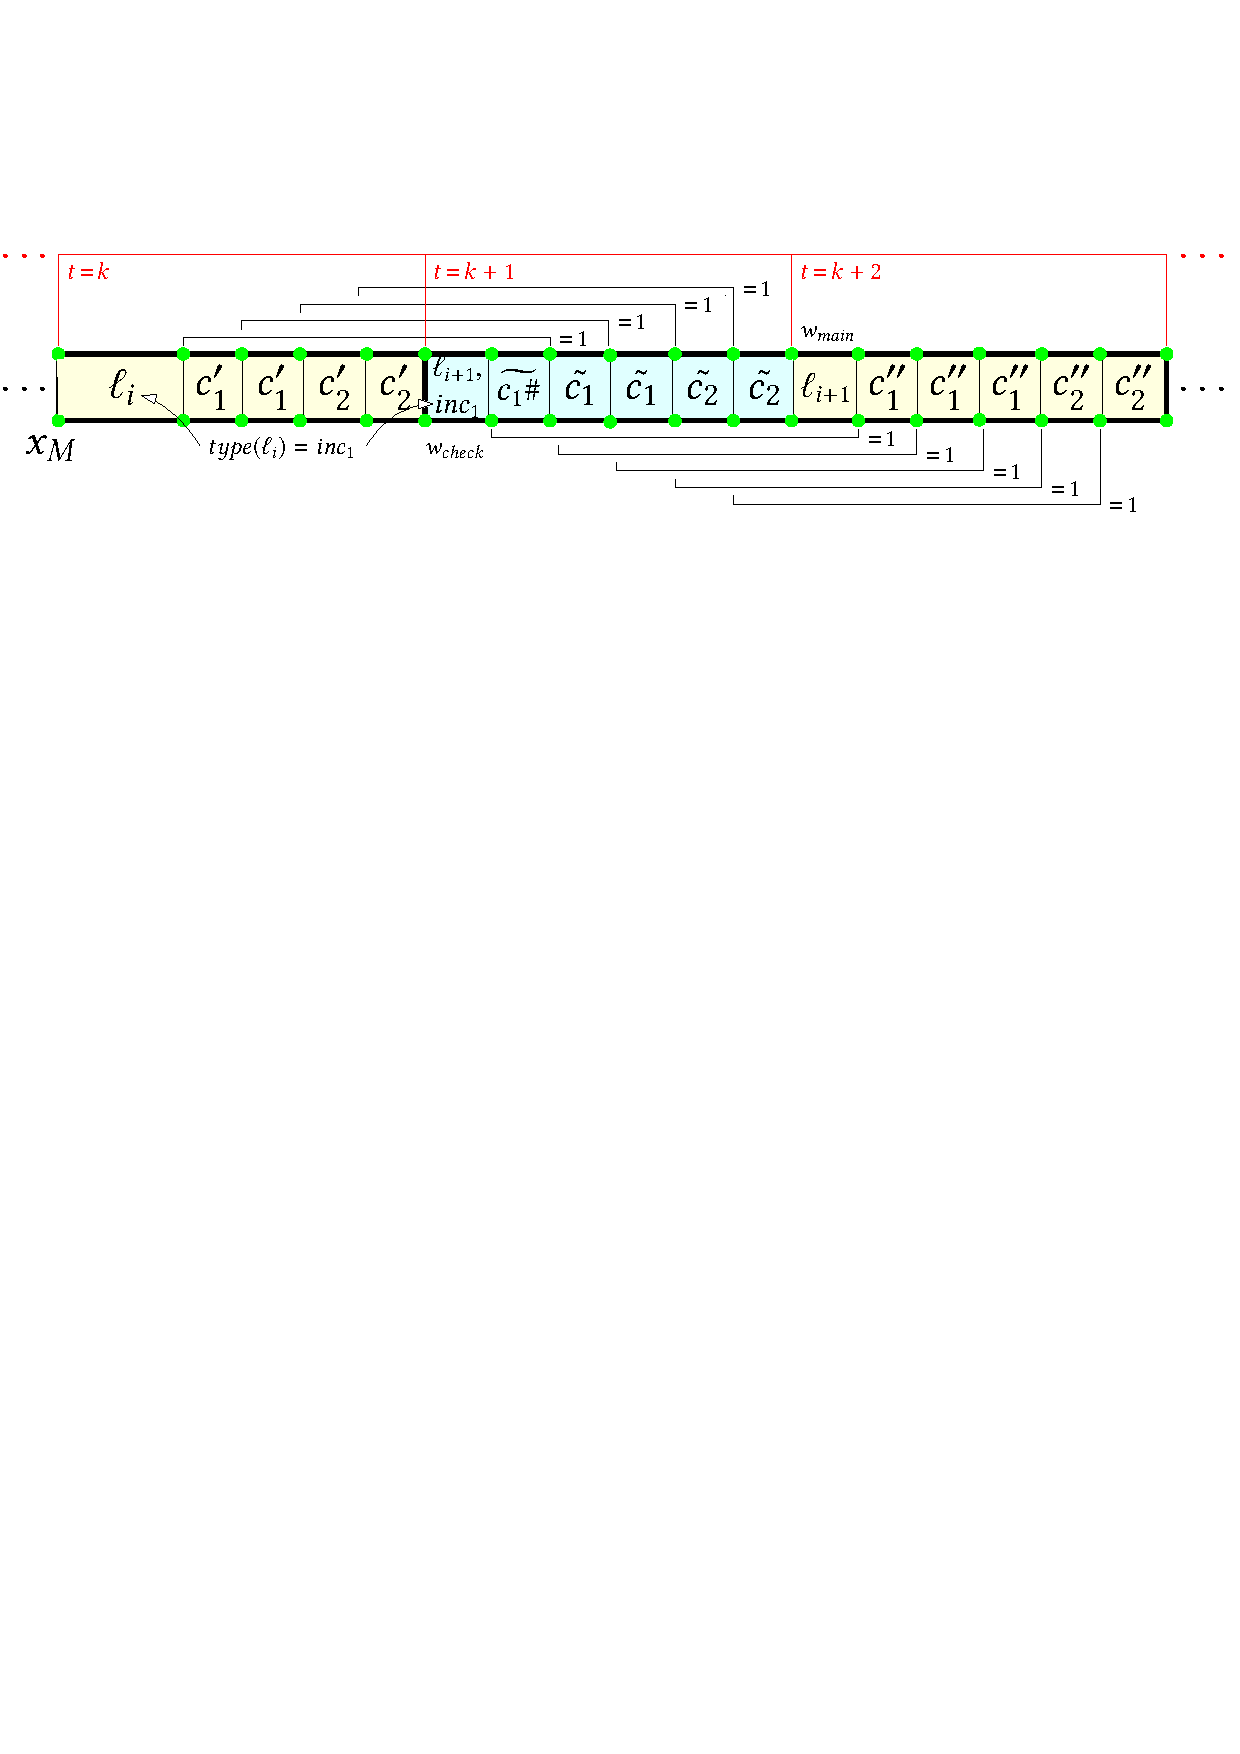
\includegraphics[width=\textwidth]{Chaps/Timelines/counters.pdf}
    \caption{
%  
A fragment of a computation code with a configuration code for 
an instruction $\ell_{i+1}$. Main-codes are highlighted in yellow and check-codes in cyan. Each square can also be seen as a token of a timeline for $x_M$ (tokens are decorated with their start time and their temporal constraints).
%%Encoding of a computation of $M$ as a timeline for $x_M$. 
%%We focus on the (simpler) case of increment instructions. 
%%A computation is given by the concatenation of main-codes (highlighted in yellow) and check-codes (in cyan). The first character (token) of a main-code is an instruction label, whereas the first character of a check-code is an instruction label, 
%%along with the type of the previous instruction (in the figure, $inc_1$ stands for an instruction incrementing $c_1$). 
%%The values of $c_1$ and $c_2$ are represented by the number of occurrences of tokens $c_1$ and $c_2$ respectively. 
%%Any check-code must have the same instruction label as the main-code \emph{following} it, and encode the same configuration.
%At every integer instant of time, we force some check- or main-code to begin. 
%
%%In order to ensure that a check-code $w_{check}$ represents the same value of $c_1$ (resp., $c_2$) as the following main-code $w_{main}$, we put into one-to-one correspondence an occurrence of $c_1$ (resp., $c_2$) in $w_{check}$ and one in $w_{main}$. To enforce this, the start time/point of each occurrence of $c_1$ (resp., $c_2$) in $w_{check}$ must be followed, \emph{after exactly 1 instant of time}, by the start time/point of the (corresponding) occurrence of $c_1$ (resp., $c_2$) in $w_{main}$ (as in the case of Metric Temporal Logic, singular intervals play a fundamental role here).
%To manage the increment of 1 unit of $c_1$, we force the same correspondence among \emph{unmarked} (i.e., without \#) occurrences of $c_1$ in $w_{check}$ and those of the \emph{preceding} main-code. There is a single token $c_1\#$ in $w_{check}$---that represents the unit added to $c_1$ by the instruction $\ell_i$---which does not correspond to any of the $c_1$'s of the preceding main-code. 
%%Let us observe that, since the time domain is \emph{dense}, in check-codes we can always add some more marked units $c_1\#$ in between the instruction label and the first unmarked occurrence of $c_1$.     
%    
In the figure, for $h\in\{1,2\}$, the symbols $c_h'$, $\tilde{c_h}$, $\widetilde{c_h\#}$, and $c_h''$, stand respectively for $(\ell_i ,c_h)$, $(\ell_{i+1},inc_1,c_h)$, $(\ell_{i+1},inc_1,(c_h,\#))$, and $(\ell_{i+1} ,c_h)$.
    }
    \label{fig:counters}
\end{figure}
A \emph{computation}-code is a %non-empty
sequence of configuration-codes $\pi= w_{\Checking}^{1}\cdot w_\main^{1}\cdots\allowbreak  w_{\Checking}^{n}\cdot w_\main^{n}$ such that, for all $1\leq j<n$, the following holds (we assume $\ell_i$ to be the instruction label associated with the configuration code $w_{\Checking}^{i}\cdot w_\main^{i}$):
%
\begin{itemize}
  \item $\ell_j\neq \ell_\halt$;
  \item if $\ell_j\in\Inc$ with $c(\ell_j)=c_h$, then $\ell_{j+1}=\Succ(\ell_j)$ and  $w_{\Checking}^{j+1}$ is associated with the operation
  $\inc_h$;
  \item if $\ell_j\in\Dec$ with $c(\ell_j)=c_h$, and the first symbol of $w_\main^{j}$ is $(\ell_j,\zero(\ell_j))$ (resp., $(\ell_j,\dec(\ell_j))$),
  then $\ell_{j+1}=\zero(\ell_j)$ (resp., $\ell_{j+1}=\dec(\ell_j)$) and  $w_{\Checking}^{j+1}$ is associated with the operation
  $\zero_h$ (resp., $\dec_h$).
\end{itemize}
%
The computation-code $\pi$ is \emph{well-formed} if, additionally, each configuration-code in $\pi$ is \emph{well-formed} and, for all $1\leq j<n$, the following holds  (we assume  $(\ell_i,n_1^{i},n_2^{i})$
to be the configuration encoded by $w_{\Checking}^{i}\cdot w_\main^{i}$):
%
\begin{itemize}
  \item if $\ell_j\in\Inc$, with $c(\ell_j)=c_h$,  then $n_h^{j+1}= n_h^{j}+1$ and $n_{3-h}^{j+1}= n_{3-h}^{j}$;
  \item if $\ell_j\in\Dec$, with $c(\ell_j)=c_h$, then $n_{3-h}^{j+1}= n_{3-h}^{j}$. Moreover, if  $w_{\Checking}^{j+1}$ is associated with %the operation
  $\dec_h$, then $n_h^{j+1}= n_h^{j}-1$.
\end{itemize}
%
Clearly, a well-formed computation code  $\pi$ encodes a computation of the Minsky 2-counter machine. 

A computation-code $\pi$ is \emph{initial} if it starts with the  prefix $(\ell_\init,\zero_1)\cdot  \ell_\init$, and it is \emph{halting} if it leads to a configuration-code associated with the halting label $\ell_\halt$. The counter machine $M$ halts if and only if there is an initial and halting well-formed computation-code.

\paragraph*{Definition of $x_M$ and $R_M$.}
Let us show now how to reduce the problem of checking the existence of an initial and halting well-formed computation-code to a TP problem for the state variable $x_M$. 

The idea is to define a timeline where the sequence of values of its tokens is a well-formed computation-code. The durations of tokens are suitably exploited to guarantee well-formedness of computation-codes. We refer the reader again to Figure~\ref{fig:counters} for an intuition. 
Each symbol of the computation-code is associated with a token having a positive duration. The overall duration of the sequence of tokens corresponding to a check-code or a main-code amounts exactly to one time unit. To allow for the encoding of 
%possibly unbounded 
arbitrarily large values of counters in one time unit, the duration of such tokens is not fixed (taking advantage of the dense temporal domain). In two adjacent check/main-codes, the time elapsed between the start times of corresponding elements in the representation of the value of a counter (see elements in Figure~\ref{fig:counters} connected by horizontal lines) amounts exactly to one time unit. Such a constraint allows us to compare the values of counters in adjacent codes, either checking for equality, or simulating (by using marked symbols) increment and decrement operations. Note that there is a single \emph{marked} token $c_1$ in the check-code---that represents the unit added to $c_1$ by the instruction $\ell_i$---which does not correspond to any of the $c_1$'s of the preceding main-code.

We now formally define a state variable $x_M$ and a set $R_M$ of synchronization rules for $x_M$ such that the untimed part of any timeline (i.e., neglecting tokens' durations)
for $x_M$ satisfying the rules in $R_M$ is (represents) an initial and halting well-formed computation-code. Thus, $M$ halts if and only if there exists a timeline for $x_M$ satisfying the rules in $R_M$.

As for $x_M$, we let $x_M= (V,T,D)$ where, for each $v\in V$, 
%we have 
$D(v)=\mathopen]0,1\mathclose]$. This sets the \emph{strict time monotonicity} constraint, namely, the duration of a token along a timeline is always greater than zero and less than or equal to 1. 

The value transition function $T$ of $x_M$ ensures the following requirement.
\begin{claim}\label{ref:claim}
The untimed part of any timeline for $x_M$ whose first token has value $(\ell_\init,\zero_1)$
 is a prefix of some initial computation-code. Moreover, $(\ell_\init,\zero_1)\notin T(v)$ for all $v\in V$.
\end{claim}
It is a straightforward task to define $T$ in  such a way that the previous requirement is fulfilled (for details, see Appendix~\ref{sec:undecidabilityTrans}).
 
Finally, the synchronization rules in $R_M$ ensure the following requirements.
%
 \begin{itemize}
%   \item \emph{Strict time monotonicity:}  the duration of a token along a timeline is always greater
%   than zero and less or equal to 1. This is expressed by the following rules: for all $v\in V$, 
%   %
%   $
%   o[x_M=v] \rightarrow o\leq^{\start,\End}_{(0,1]} o 
%   $.
%   %
   \item \emph{Initialization:} every timeline starts with two tokens, the first one having value
   $(\ell_\init,\zero_1)$, and the second having value $\ell_\init$. By Claim~\ref{ref:claim} and the fact that no instruction
   of $M$ leads to $\ell_\init$, it suffices to require that a timeline has a token with value $(\ell_\init,\zero_1)$ and a token with value
   $\ell_\init$.
   This is ensured by the following two trigger-less rules:
   %
   \[
   \true \rightarrow \exists \, o[x_M=(\ell_\init,\zero_1)].\, \true
   \] and \[
   \true \rightarrow \exists \, o[x_M= \ell_\init].\, \true
   .\]
   %
   \item \emph{Halting:} every timeline leads to a configuration-code associated with the halting label. By the rules for initialization and Claim~\ref{ref:claim}, it suffices to require that a timeline has a token with value $\ell_\halt$. This is ensured by the following trigger-less rule:
   %
   \[
   \true \rightarrow \exists \, o[x_M=\ell_\halt].\, \true
   .\]
   %
    %
   \item \emph{1-Time distance between consecutive control values:} a \emph{control $V$-value} corresponds to the first symbol of a $\main$-code or a $\Checking$-code, i.e., it is an element in $V\setminus (V_{c_1}\cup V_{c_2})$. We require  that the difference of the start times of two consecutive tokens along a timeline having a control $V$-value is exactly $1$. Formally, 
%      in other terms, 
    for each pair $tk$ and $tk'$ of tokens along a timeline such that $tk$ and $tk'$ have a control $V$-value, $tk$ precedes $tk'$, and there is no token between $tk$ and $tk'$ having a control $V$-value, it holds that $\startTime(tk')-\startTime(tk)=1$ (we write this with a little abuse of notation). By Claim~\ref{ref:claim}, strict time monotonicity, and the halting requirement, it suffices to ensure that each token $tk$ having a control $V$-value distinct from $\ell_\halt$ is eventually followed by a token $tk'$ such that $tk'$ has a control $V$-value and $\startTime(tk')-\startTime(tk)=1$. To this aim, for each  $v\in V_\Con\setminus \{\ell_\halt\}$, being $V_\Con$ the set of control $V$-values,  we write the following trigger rule:
    %
   \[
   o[x_M=v] \rightarrow \displaystyle{\bigvee_{u\in V_\Con}} \exists\, o'[x_M= u].\, o\leq^{\start,\start}_{[1,1]} o'. 
   %\\ \text{for each } v\in V_\Con\setminus \{\ell_\halt\}.
   \]
   
   \item \emph{Well-formedness of configuration-codes:} we need to guarantee that for each configuration-code $w_\Checking\cdot w_\main$ occurring along a timeline and 
%for 
    each counter $c_h$, the value of $c_h$ along the $\main$-code $w_\main$ and the $\Checking$-code $w_\Checking$ coincide.
    By Claim~\ref{ref:claim}, strict time monotonicity, initialization, and 1-Time distance between consecutive control values,  it suffices to ensure that $(i)$~each token $tk$  with
    a $V_{c_h}$-value in $V_\Checking$ is eventually followed by a token $tk'$ with a $V_{c_h}$-value such that  $\startTime(tk')-\startTime(tk)=1$, and vice versa $(ii)$~each token $tk$  with
    a $V_{c_h}$-value in $V_\main$ is eventually preceded by a token $tk'$ with a $V_{c_h}$-value such that  $\startTime(tk)-\startTime(tk')=1$. As for the former requirement, for each   $v\in V_{c_h}\cap V_\Checking$, we write the rule:
    %
   \[
   o[x_M=v] \rightarrow \displaystyle{\bigvee_{u\in V_{c_h}}} \exists\, o'[x_M= u].\, o\leq^{\start,\start}_{[1,1]} o'.
   %\\ \text{for each }  v\in V_{c_h}\cap V_\Checking.
   \]
   
   For the latter, for each   $v\in V_{c_h}\cap V_\main$, we have the rule:
       %
   \[
   o[x_M=v] \rightarrow \displaystyle{\bigvee_{u\in V_{c_h}}} \exists\, o'[x_M= u].\, o'\leq^{\start,\start}_{[1,1]} o.
   %\\ \text{for each } v\in V_{c_h}\cap V_\main.
   \]
   
   \item \emph{Increment and decrement:} we need to guarantee that the increment and decrement instructions are correctly simulated.
    By Claim~\ref{ref:claim} and the previously defined synchronization rules, we can assume that the untimed part $\pi$ of a timeline is an initial and halting
    computation-code such that all  configuration-codes occurring in $\pi$ are well-formed.

    Let $w_\main \cdot w_\Checking$ be a subword occurring in $\pi$ such that
    $w_\main$ (resp., $w_\Checking$) is a $\main$-code (resp., $\Checking$-code). Let $\ell_\main$ (resp., $\ell_\Checking$) be the instruction label
    associated with $w_\main$ (resp., $w_\Checking$) and for $i=1,2$, let $n_i^{\main}$ (resp., $n_i^{\Checking}$) be the value of counter $c_i$ encoded by
     $w_\main$ (resp., $w_\Checking$). Let $c_h=c(\ell_\main)$. By construction $\ell_\main\neq \ell_\halt$, end either $\ell_\main\in\Inc$   and
     $\ell_\Checking =\Succ(\ell_\main)$, or $\ell_\main\in \Dec$  and $\ell_\Checking\in \{\zero(\ell_\main),\dec(\ell_\main)\}$. Moreover, if $\ell_\main\in \Dec$
     and $\ell_\Checking = \zero(\ell_\main)$, then $n_h^{\Checking}= n_h^{\main}=0$.
     Thus, it remains to ensure the following two requirements:
     \begin{itemize}
       \item[(*)] if $\ell_\main\in\Inc$, then $n_h^{\Checking}= n_h^{\main}+1$ and $n_{3-h}^{\Checking}= n_{3-h}^{\main}$;
       \item[(**)] if $\ell_\main\in\Dec$, then $n_{3-h}^{\Checking}= n_{3-h}^{\main}$, and whenever
       $\ell_\Checking = \dec(\ell_\main)$, then $n_h^{\Checking}= n_h^{\main}-1$.
     \end{itemize}

First we observe that, if $\ell_\main\in\Inc$, our encoding ensures that all $V_{c_{3-h}}$-values in $w_\main$ and in $w_\Checking$ are unmarked,
all $V_{c_{h}}$-values in  $w_\main$ are unmarked, and there is exactly one marked $V_{c_{h}}$-value  in  $w_\Checking$.
If instead $\ell_\main\in\Dec$, our encoding ensures that all $V_{c_{3-h}}$-values in $w_\main$ and in $w_\Checking$ are unmarked,
all $V_{c_{h}}$-values in  $w_\Checking$ are unmarked, and in case $\ell_\Checking= \dec(\ell_\main)$, then there is exactly one marked $V_{c_{h}}$-value  in  $w_\main$.
Thus, by strict time monotonicity and 1-Time distance between consecutive control values, it follows that requirements~(*) and~(**) are captured by the following
rules, where $U_{c_i}$ denotes the set of \emph{unmarked} $V_{c_i}$-values, for $i=1,2$, and $V_\init$ (resp., $V_\halt$) is the set of $V$-values associated with the label $\ell_\init$ (resp., $\ell_\halt$). For each   $v\in (U_{c_i}\cap V_\main)\setminus V_\halt$, we have the rule:
 %
   \[
   o[x_M=v] \rightarrow \displaystyle{\bigvee_{u\in U_{c_i}}} \exists\, o'[x_M= u].\, o\leq^{\start,\start}_{[1,1]} o'. 
   %\\ \text{for each }  v\in (U_{c_i}\cap V_\main)\setminus V_\halt
   \]
   
   For each $v\in (U_{c_i}\cap V_\Checking)\setminus V_\init$, we have the rule:
   \[
   o[x_M=v] \rightarrow \displaystyle{\bigvee_{u\in U_{c_i}}} \exists\, o'[x_M= u].\, o'\leq^{\start,\start}_{[1,1]} o .
   %\\ \text{for each } v\in (U_{c_i}\cap V_\Checking)\setminus V_\init \qedhere
   \]
 \end{itemize}
This concludes the proof of the theorem.
\end{proof}

It is worth observing that all the above trigger rules are \emph{simple}, hence \emph{undecidability of the TP problem holds also under the restriction to simple trigger rules}.

In order to ensure the well-formedness of configuration-codes and the increment/decrement requirements, a one-to-one correspondence between (suitable) pairs of tokens in main- and check-codes is enforced thanks to the above trigger rules. Whereas most of such rules are (already) satisfied under the future semantics (as the extra conjoined atoms added by Definition~\ref{def:futurerules} would be \lq\lq subsumed\rq\rq\ by already-existing ones), some rules are not (the second ones of the well-formedness and increment/decrement requirements are unsatisfiable under the future semantics). 
As a result, intuitively, having only rules under the future semantics,
we can only force the presence, for every token with value $c_h$ (for $h=1,2$), of another token with value $c_h$ starting exactly one time instant later, in the following main-/check-code. However, we cannot prevent extra \lq\lq spurious\rq\rq\  tokens to appear moving from a code to the following one.
This is the reason why, with only rules under the future semantics, we lose the ability of encoding computations of (exact) Minsky machines. Only \emph{gainy counter machines}~\cite{DemriL09}---a variant of Minsky machines whose counters may \lq\lq erroneously\rq\rq\ increase---can be captured, thus proving, as a consequence, 
\emph{non-primitive recursive-hardness} of the future TP problem (the halting problem for gainy counter machines is known to be non-primitive recursive~\cite{DemriL09}). 

\begin{theorem}\label{theorem:NPRHardness}
The future TP problem, even with \emph{one state variable}, is non-primitive recursive-hard also under one of the following two assumptions: \emph{either} $(1)$ the trigger rules are simple,
\emph{or} $(2)$ the intervals are in $\Intv_{(0,\infty)}$%
\footnote{We refer to intervals in rules' atoms and in the constraint functions of state variables.}.
\end{theorem}

Since this result is just an adaptation of the previous one (apart from some technicalities), we report its proof in Appendix~\ref{sec:NPRHardness}. 
%As we show there, 
%non-primitive recursive-hardness holds also with just one state variable, and again with the restriction to simple trigger rules.

In the next section, we will show that future TP with simple trigger rules is indeed decidable in non-primitive recursive time. 
\section{Decidability of future TP with simple trigger rules}\label{sec:DecisionProcedures}

In this section, we show that the decidability of the TP problem can be recovered assuming that the trigger rules are \emph{simple} and \emph{interpreted under the future semantics}. Moreover, under the additional assumption that intervals in trigger rules are non-singular (respectively, are in $\Intv_{(0,\infty)}$), the problem is
in $\EXPSPACE$ (respectively, in $\Psp$). 
%
The decidability status of \emph{future TP with arbitrary trigger rules remains an open problem}.
% As already mentioned, in Section~\ref{sec:NPRHardness}, we prove that such problem is non-primitive recursive-hard even if $(i)$~all the trigger rules are simple or $(ii)$~intervals in rule' atoms and in the constraint functions of the state variables
% are assumed to be in $\Intv_{(0,\infty)}$.

The rest of this section is organized as follows: in Section~\ref{sec:TimedAutomata}, we recall Timed Automata (\TA)~\cite{ALUR1994183}  and Metric Temporal logic (\MTL)~\cite{Koymans90}. In Section~\ref{sec:Reduction}, we reduce the future TP problem
with simple trigger rules to the \emph{existential MC problem} for \TA s against \MTL\ over \emph{finite timed words}. The latter problem is known to be decidable~\cite{OuaknineW07}.


\subsection{Timed automata and the logic \MTL}\label{sec:TimedAutomata}

We start by recalling the notion of timed automaton (\TA)~\cite{ALUR1994183} and the logic \MTL~\cite{Koymans90}.

Let $\Sigma$ be a finite alphabet. A  \emph{timed word} $w$ over  $\Sigma$ is
a \emph{finite}  word $w=(a_0,\tau_0)\cdots (a_n,\tau_n)$ over $\Sigma\times \RealP$ %(intuitively, %for each $i$,
($\tau_i$ is called a \emph{timestamp}, and intuitively represents the time at which the \lq\lq event\rq\rq\ $a_i$ occurs) such that  $\tau_{i}\leq \tau_{i+1}$ for all $0\leq i<n$ (\emph{monotonicity} requirement).
The timed word $w$ is also denoted by $(\sigma,\tau)$, where $\sigma$ is the finite (untimed) word $a_0 \cdots a_n$
and $\tau$ is the sequence of timestamps $\tau_0, \ldots, \tau_n$.
A \emph{timed language}  over $\Sigma$ is a set of timed words over $\Sigma$.%\vspace{0.2cm}

\paragraph{Timed Automata (\TA).} Let $C$ be a finite set of clocks. A clock valuation $\val:C\to \RealP$ for $C$ is a function
 assigning a non-negative real value to each clock in $C$.
Given a value $t\in\RealP$ and a set $\Res\subseteq C$ (that we call \emph{reset set}), $(\val+ t)$ and $\val[\Res]$ denote the valuations for $C$ defined respectively as follows: for all $c\in C$,
 $(\val +t)(c) = \val(c)+t$, and $\val[\Res](c)=0$ if $c\in \Res$ and $\val[\Res](c)=\val(c)$ otherwise.

 A \emph{clock constraint} $\theta$ over $C$ is a Boolean combination of atomic formulas of the form
$c \in I$ or $c-c'\in I$, where $c,c'\in C$ and
$I\in\Intv$.
Given a clock valuation $\val$ and a clock constraint $\theta$, $\val$ is said to satisfy $\theta$, written
$\val\models \theta$, if 
$\theta$ evaluates to true after replacing each occurrence of a clock $c$ in $\theta$ by $\val(c)$, and interpreting Boolean connectives and membership to intervals in the standard way. 
% for each conjunct $c\in I$ (respectively, $c-c'\in I$) of $\theta$, it holds $\val(c)\in I$ (respectively, $\val(c)-\val(c')\in I$).
%
We denote by $\Phi(C)$ the set of all possible clock constraints over $C$.

\begin{definition}[Timed automaton \TA]
 A  \TA\ over  $\Sigma$ is a tuple
$\Au=\tpl{\Sigma, Q,q_0,C,\Delta,F}$, where $Q$ is a finite
set of (control) states, $q_0\in Q$ is the initial
state, $C$ is a finite set of clocks,
$F\subseteq Q$ is the set of accepting states, and $\Delta \subseteq Q\times \Sigma \times \Phi(C) \times 2^{C} \times Q $ is the transition relation.

The \emph{maximal constant of $\Au$} is the greatest integer occurring as an endpoint of some interval in the clock constraints of the transitions of $\Au$.
\end{definition}

Intuitively, in a \TA\  $\Au$, while transitions are instantaneous, time can elapse in a control
state. The clocks  progress at the same speed  and can
be reset independently of each other when a transition is executed, in such a way that each clock
keeps track of the time elapsed since the last reset. Moreover, clock constraints
are used as guards of transitions to restrict the behavior of the
automaton.

A configuration of $\Au$ is a pair $(q,\val)$, where $q\in Q$ and $\val$ is a clock valuation for $C$.
A run $r$ of $\Au$ on a timed word $w=(a_0,\tau_0)\cdots (a_n,\tau_n)$ over $\Sigma$
is a sequence  of configurations
 $r=(q_0,\val_0)\cdots (q_{n+1},\val_{n+1})$ starting at the initial configuration $(q_0,\val_0)$,
where $\val_0(c)=0$ for all $c\in C$ (\emph{initiation requirement}), and 
\begin{itemize}
\item for all $0\leq i\leq n$ we have (\emph{consecution requirement}): 
  $(i)$~\mbox{$(q_{i},a_i,\theta,\Res,q_{i+1})\!\in\!\Delta$} for some $\theta\in\Phi(C)$ and reset set $\Res$, $(ii)$~$(\val_{i} +\tau_i-\tau_{i-1})\models \theta$ and $(iii)$~$\val_{i+1}= (\val_{i} +\tau_i-\tau_{i-1})[\Res]$ (we let $\tau_{-1}=0$).
\end{itemize}
The intuitive behavior of the \TA\ $\Au$ is the following.
Assume that $\Au$ is on state $q\in Q$ after reading the symbol $(a',\tau_i)$ at time $\tau_i$ and, 
at that time, the clock valuation is $\val$. On reading 
$(a,\tau_{i+1})$, $\Au$ chooses a transition of the form $\delta=(q,a,\theta,\Res, q')\in
\Delta$ such that the constraint $\theta$
is fulfilled by $(\val+t)$, with
%where $\sval$ is the clock valuation before taking $\delta$, 
$t=\tau_{i+1}-\tau_{i}$. 
The control then changes from $q$ to $q'$ and $\val$ is updated 
in such a way as to record the amount of time elapsed $t$ in the clock valuation, and to reset the clocks in $\Res$,
namely, $\val$ is updated to $(\val +t)[\Res]$.

A run $r$ is \emph{accepting} if $q_{n+1}\in F$.
The \emph{timed language} $\TLang(\Au)$ of $\Au$ is the set of  timed words $w$ over $\Sigma$
such that there is an accepting run of $\Au$ on $w$.

As shown in~\cite{ALUR1994183}, given two \TA s $\mathcal{A}_1$, with $s_1$ states and $k_1$ clocks, and $\mathcal{A}_2$, with $s_2$ states and $k_2$ clocks, the union (resp., intersection) automaton $\mathcal{A}_\vee$ (resp., $\mathcal{A}_\wedge$) such that $\TLang(\mathcal{A}_\vee)=\TLang(\mathcal{A}_1)\cup\TLang(\mathcal{A}_2)$ (resp., $\TLang(\mathcal{A}_\wedge)=\TLang(\mathcal{A}_1)\cap\TLang(\mathcal{A}_2)$) 
can be effectively calculated, and 
has $s_1+s_2$ states (resp., $s_1\cdot s_2$ states) and $k_1+k_2$ clocks (resp., $k_1+k_2$ clocks).

\paragraph{The logic \MTL.}Let us now recall the framework of Metric Temporal Logic (\MTL)~\cite{Koymans90},  a well-known  timed linear-time temporal logic which extends standard \LTL\ with time
constraints on the until modality.

Given a finite set $\Prop$ of proposition letters, the set of \MTL\ formulas $\varphi$ over $\Prop$ is defined by the following grammar:
%
\[
\varphi::= \top \mid
p \mid
\varphi \vee \varphi \mid
\neg \varphi      \mid
\varphi \StrictUntil_I\varphi,
\]
%
where $p\in \Prop$, $I\in\Intv$, and
$\StrictUntil_I$  is the \emph{strict timed until} \MTL\ modality. 

\MTL\ formulas over $\Prop$ are interpreted over  timed words over $2^{\Prop}$.
Given an \MTL\ formula $\varphi$, a  timed word $w=(\sigma,\tau)$ over $2^{\Prop}$, and a position $0\leq  i< |w|$, the satisfaction relation
$(w,i)\models\varphi$---meaning that $\varphi$ holds at position $i$ of $w$---is  defined as follows (we omit the clauses for Boolean connectives):
\begin{itemize}
\item $(w,i)\models p \iff p\in\sigma(i)$,
\item $(w,i)\models \varphi_1 \StrictUntil_I\varphi_2
              \iff $ there exists $j>i$ such that $(w,j)\models \varphi_2$, $\tau_j-\tau_i\in I$, and $(w,k)\models \varphi_1$ for all $i<k<j$.
\end{itemize}
%
A \emph{model of $\varphi$} is a  timed word $w$ over $2^{\Prop}$ such that $(w,0)\models \varphi$. The \emph{timed language} $\TLang(\varphi)$ of $\varphi$ is the set of  models of $\varphi$.

The \emph{existential MC problem for \TA s against \MTL} is the problem of checking, for a given \TA\ $\Au$ over $2^{\Prop}$ and an \MTL\ formula $\varphi$ over $\Prop$, whether
$\TLang(\Au)\cap \TLang(\varphi)\neq \emptyset$.

In \MTL, we use standard shortcuts such as: $\Eventually_I \varphi$ for $\varphi \vee (\true 
\StrictUntil_I \varphi)$ (\emph{timed eventually} or \emph{timed future}), and $\Always_I \varphi$ for $\neg \Eventually_I  \neg\varphi$ (\emph{timed always} or \emph{timed globally}).
 
 We also consider two fragments of \MTL, namely, \MITL\ (Metric Interval Temporal Logic)
and $\MITLR$~\cite{Alur:1996}: \MITL\ is obtained by allowing only non-singular intervals of $\Intv$ at the subscript of $\StrictUntil$, while $\MITLR$ is the fragment of \MITL\ obtained by allowing only intervals
in $\IntvR$. 

The \emph{maximal constant} of an \MTL\ formula $\varphi$ is the greatest integer occurring as an endpoint of some interval of (the occurrences of) the $\StrictUntil_I$ modality in $\varphi$.

\subsection{Reduction to existential MC for \TA s against \MTL}\label{sec:Reduction}
We now solve the future TP problem with simple trigger rules by means of an exponential-time reduction to the existential MC problem for \TA s against \MTL. 

In the following, we fix an instance $P=(SV,R)$ of the problem where the trigger rules in $R$ are simple. The \emph{maximal constant} of $P$, denoted by $K_P$, is the greatest integer occurring in the atoms of the rules in $R$ and in the constraint  functions of the state variables in $SV$.

The proposed reduction consists of three steps:
\begin{enumerate}
  \item first, we define an encoding of the multi-timelines of $SV$ by means of timed words over $2^{\Prop}$ for a suitable finite set $\Prop$ of proposition letters,
  and show how to construct a \TA\ $\Au_{SV}$ over $2^{\Prop}$ accepting such encodings;
  \item next, we build an \MTL\ formula $\varphi_{\forall}$ over $\Prop$ such that for each multi-timeline $\Pi$ of $SV$ and encoding $w_\Pi$ of $\Pi$, $w_\Pi$ is a model of $\varphi_\forall$
  if and only if $\Pi$ satisfies all the trigger rules in $R$ under the future semantics;
  \item finally, we construct a \TA\ $\Au_{\exists}$ over $2^{\Prop}$ such that for each multi-timeline $\Pi$ of $SV$ and encoding $w_\Pi$ of $\Pi$, $w_\Pi$ is accepted by $\Au_{\exists}$
  if and only if $\Pi$ satisfies all the trigger-less rules in $R$.
\end{enumerate}
Hence, there is a future plan for $P=(SV,R)$  iff  $\TLang(\Au_{SV})\cap \TLang(\Au_\exists )\cap \TLang(\varphi_\forall)\neq \emptyset$. %We now proceed with the technical details.


For each $x\in SV$, we let $x=\tpl{V_x,T_x,D_x}$.
Given an interval $I\in\Intv$ and a natural number $n\in \Nat$, let $n+I$ (respectively, $n-I$) denote the set of non-negative real numbers
$\tau\in\RealP$ such that $\tau-n\in I$ (respectively, $n-\tau \in I$). Note that $n+I$ (respectively, $n-I$) is a (possibly empty) interval in $\Intv$ whose endpoints can be trivially calculated.

For an atom $\rho$ in $R$ involving a time constant (time-point atom), let $I(\rho)$ be the interval in $\Intv$ defined as follows:
\begin{itemize}
  \item if $\rho$ has the form  $o\leq^{e}_{I} n$ (resp., $n\leq^{e}_{I} o$), then $I(\rho)= n-I$ (resp., $I(\rho)= n+I$).
\end{itemize}
We finally define $\Intv_R$ as the set of intervals $J\in\Intv$ such that $J=I(\rho)$ for some time-point atom $\rho$ occurring in a trigger rule of  $R$.


\paragraph{Encodings of multi-timelines of $SV$.} We assume that for distinct state variables $x$ and $x'$, the sets $V_x$ and  $V_{x'}$
are disjoint. We exploit the following set $\Prop$ of proposition letters to encode multi-timelines of $SV$:
\[
\Prop = \bigcup_{x\in SV}\Main_x \cup \Deriv ,
\]
\[
\Main_x = ((\{\Beg_x \}\cup V_x) \times V_x)   \cup   (V_x \times \{\End_x\}),
\]
\[
\Deriv = \Intv_R \cup \{p_>\} \cup \bigcup_{x\in SV}\bigcup_{v\in V_x}\{\Past_v^{\start},\Past_v^{\Ending}\}.
\]
Intuitively, we use the propositions in $\Main_x$ to encode a token along a timeline for $x$. The propositions in $\Deriv$, as explained below, represent
enrichments of the encoding, used for translating simple trigger rules in \MTL\ formulas under the future semantics.
 The tags $\Beg_x$ and $\End_x$ in $\Main_x$ are used to mark the start and the end of a timeline  for $x$. 
 
 A token $tk$ with value $v$ along a timeline for
 $x$ is encoded by two events: the \emph{start-event} (occurring at the start time of $tk$) and
 the \emph{end-event} (occurring at the end time of $tk$). The start-event of $tk$ is specified by a main proposition of the form
 $(v_p,v)$, where either $v_p=\Beg_x$ ($tk$ is the first token of the timeline) or $v_p$ is the value of the token for $x$
preceding $tk$. The end-event of $tk$ is instead specified by a main proposition of the form
 $(v,v_s)$, where either $v_s=\End_x$ ($tk$ is the last token of the timeline) or $v_s$ is the value of the token for $x$
following $tk$. 
%
See Figure~\ref{fig:ktimelines} for an example.
%
\begin{figure}[tb]
    \centering
    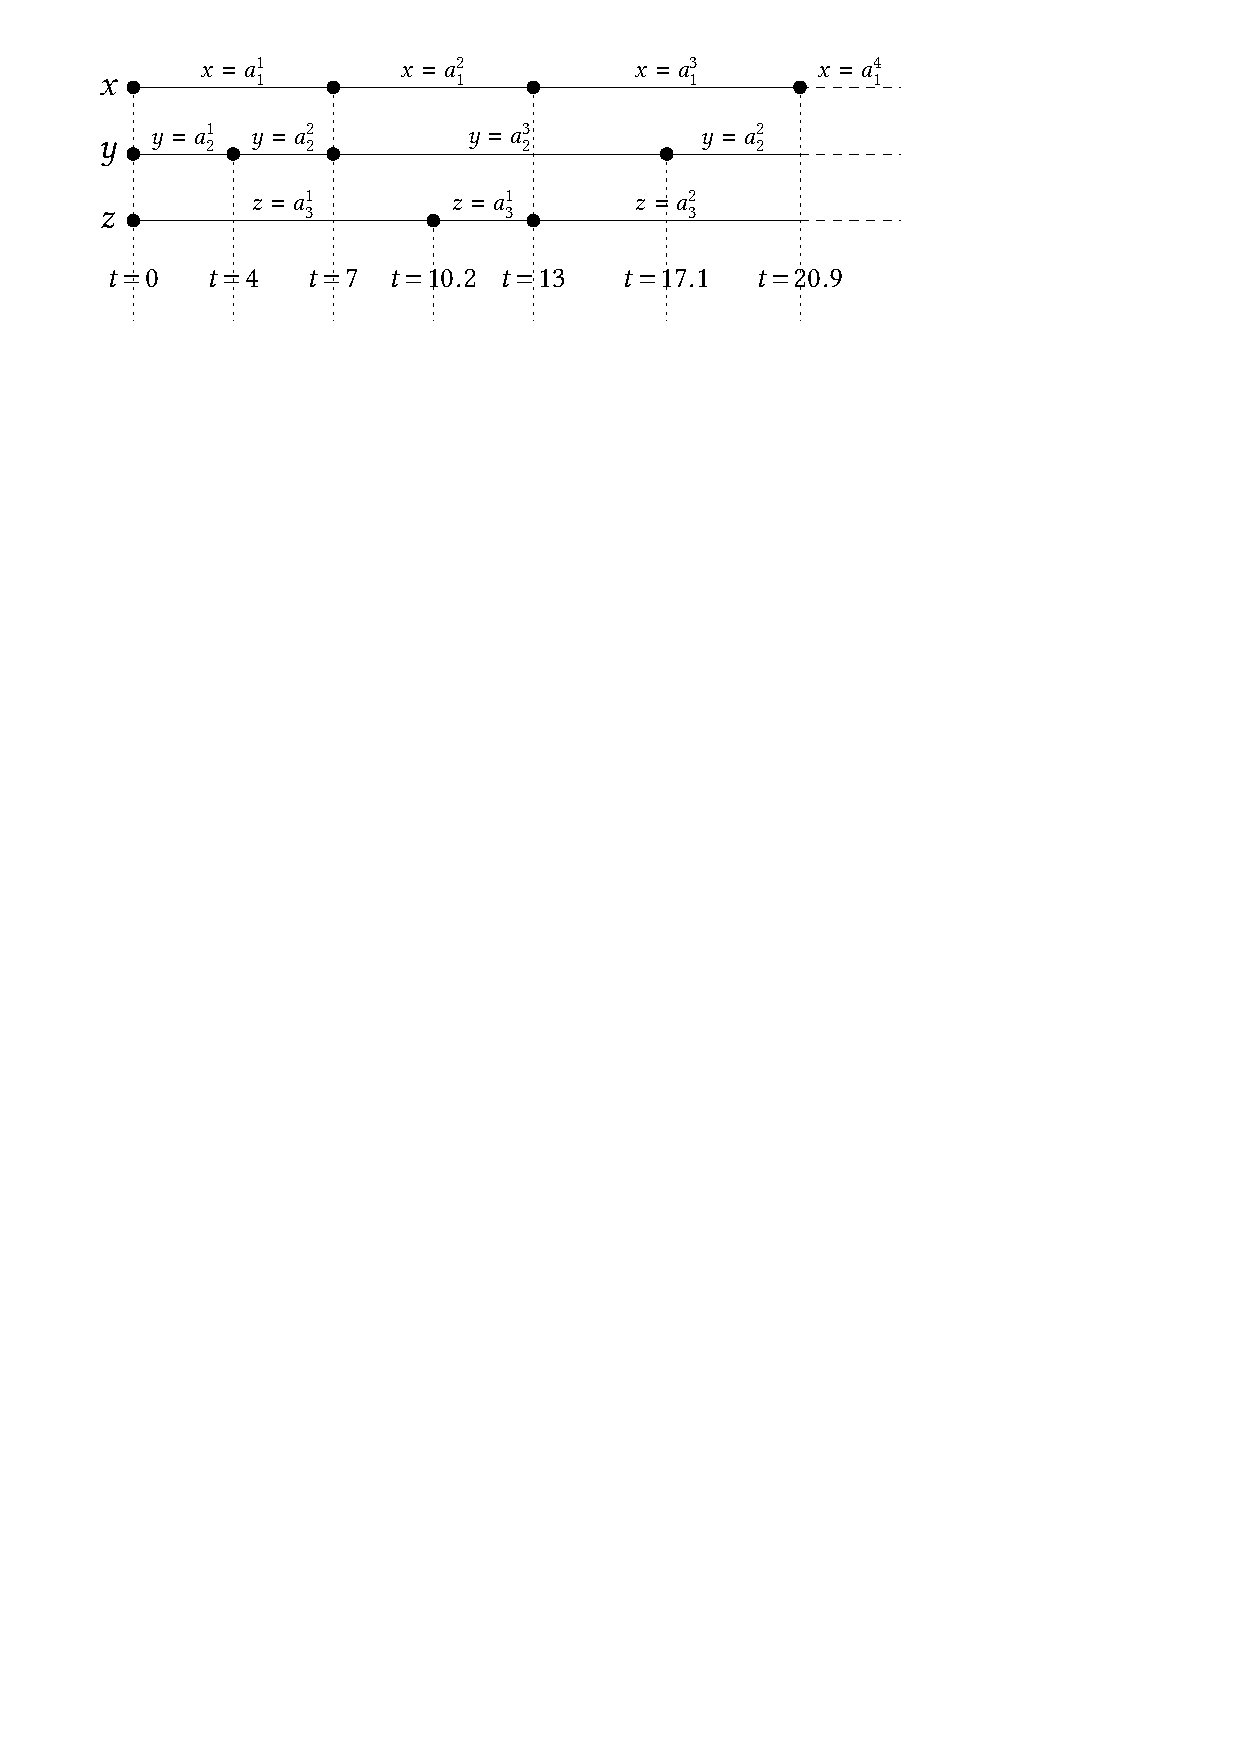
\includegraphics[width=0.85\linewidth]{Chaps/Timelines/timelineFig.pdf}
    \caption{An example of multi-timeline of $SV=\{x,y,z\}$, where in particular $V_x=\{a_1^i\mid 1\leq i\leq 4\}$, $V_y=\{a_2^i\mid 1\leq i\leq 3\}$ and $V_z=\{a_3^i\mid 1\leq i\leq 2\}$. \\
    The encoding of the timeline for $x$ depicted in the figure (we show only values in $\Main_x$) is $\big(\{(\Beg_x,a_1^1)\},0\big)\big(\{(a_1^1,a_1^2)\},7\big)\big(\{(a_1^2,a_1^3)\},13\big)\big(\{(a_1^3,a_1^4)\},20.9\big)\cdots$ \\
    The encoding of the multi-timeline of $SV$ depicted in the figure (we show only values in $\Main_x\cup\Main_y\cup\Main_z$) is $\big(\{(\Beg_x,a_1^1),(\Beg_y,a_2^1),(\Beg_z,a_3^1)\},0\big)\allowbreak
    \big(\{(a_2^1,a_2^2)\},4\big)\allowbreak
    \big(\{(a_1^1,a_1^2),(a_2^2,a_2^3)\},7\big)
    \big(\{(a^1_3,a^1_3)\},10.2\big)
    \big(\{(a_1^2,a_1^3),(a^1_3,a^2_3)\},13\big)
    \big(\{(a^3_2,a^2_2)\},17.1\big)\cdots$}
    \label{fig:ktimelines}
\end{figure}

Now we explain the meaning of the proposition letters in $\Deriv$.
The elements in  $\Intv_R$ reflect the semantics of
the time-point atoms in the trigger rules of $R$: for each $I\in \Intv_R$, $I$ holds at the current position if the current timestamp $\tau$ satisfies
$\tau\in I$.  The tag $p_>$ keeps track of whether the current timestamp is strictly greater than the previous one.
Finally,  the propositions in $\bigcup_{x\in SV}\bigcup_{v\in V_x}\{\Past_v^{\start},\Past_v^{\Ending}\}$ keep track of past token events occurring at timestamps \emph{coinciding}
with the current timestamp. 

We start by defining the encoding of timelines for $x\in SV$.
%
An \emph{encoding of a timeline for $x$} is
 a timed word $w$ over $2^{\Main_x \cup \Deriv}$ of the form
 \[
 w =(\{(\Beg_x,v_0)\}\cup S_0,\tau_0)(\{(v_0,v_1)\}\cup S_1,\tau_1)\cdots (\{(v_n,\End_x)\}\cup S_{n+1},\tau_{n+1})
 \]
 where, for all $0\leq i\leq n+1$, $S_i\subseteq \Deriv$, and % the following hold:
 \begin{itemize}
  \item $v_{i+1}\in T_x(v_i)$ for $i<n$;
 \item $\tau_0=0$ and $\tau_{i+1}-\tau_i \in D_x(v_i)$ for $i\leq n$;
  \item   $S_i\cap \Intv_R$ is the set of intervals $I\in\Intv_R$
  such that $\tau_i\in I$;
  \item $p_>\in S_i$ iff either $i=0$ or $\tau_i>\tau_{i-1}$;
  \item for all $v\in V_x$, $\Past^{\start}_v\in S_i$ (resp., $\Past^{\Ending}_v\in S_i$) iff there is $0\leq h<i$ such that $\tau_h=\tau_i$ and $v= v_h$ (resp., $\tau_h=\tau_i$, $v=v_{h-1}$ and $h>0$).
\end{itemize}
Note that the length of $w$ is at least $2$. The timed word $w$ encodes the timeline for $x$ of length $n+1$
given by $\pi=(v_0,\tau_1) (v_1,\tau_2-\tau_1)\cdots (v_n,\tau_{n+1}-\tau_n)$. Note that in the encoding, $\tau_i$ and $\tau_{i+1}$ represent the start time and the end time
of the $i$-th token of the timeline $\pi$ ($0\leq i\leq n$).
See the caption of Figure~\ref{fig:ktimelines} for an example of encoding.

Next, we define the encoding of a multi-timeline of $SV$.  For a set $P\subseteq \Prop$ and $x\in SV$, let $P[x]= P\setminus \bigcup_{y\in SV\setminus \{x\}}\Main_y$.
An \emph{encoding of a multi-timeline of $SV$} is
 a timed word $w$ over $2^{\Prop}$ of the form
$
 w =(P_0,\tau_0)\cdots (P_n,\tau_n)
$
 such that  the following conditions hold:
 \begin{itemize}
  \item  for all $x\in SV$, the timed word obtained from $(P_0[x],\tau_0)\cdots (P_n[x],\tau_n)$ by removing
  the pairs $(P_i[x],\tau_i)$ such that $P_i[x]\cap \Main_x=\emptyset$ is an encoding of a timeline for $x$;
    \item $P_0[x]\cap \Main_x\neq \emptyset$ for all $x\in SV$ (initialization).
\end{itemize}
See again Figure~\ref{fig:ktimelines} for an example of encoding of a multi-timeline.

We now construct a \TA\ $\Au_{SV}$ over $2^{\Prop}$ accepting the encodings of the multi-timelines of $SV$,
as shown in the proof of the next proposition. %, $\Au_{SV}$ uses a clock $c_x$ for each state variable  $x\in SV$ to check the time constraints on the duration of the tokens for $x$. Two additional clocks, $c_>$
%and $c_{glob}$, are exploited for capturing the meaning of the proposition $p_>$ and of the propositions in $\Intv_R$ (in particular, $c_{glob}$ is a clock which measures the current time and is never reset).

 \begin{proposition}\label{prop:AtutomataForMultiTimeline} One can construct in exponential time a \TA\ $\Au_{SV}$ over $2^{\Prop}$, with $2^{O(\sum_{x\in SV}|V_x|)}$ states, $|SV|+2$ clocks, and
 maximal constant $O(K_P)$, such that $\TLang(\Au_{SV})$ is the set of encodings of the multi-timelines of $SV$.
 \end{proposition}
 \begin{proof}
Let us fix an ordering $SV=\{x_1,\ldots,x_N\}$ of the state variables. Let $\mathcal{H}= \Deriv\setminus (\Intv_R \cup \{p_>\})$ and $V'_i = V_{x_i}\cup \{\Beg_{x_i},\End_{x_i}\}$ for all $1\leq i\leq N$.

The  \TA\ $\Au_{SV}=\tpl{2^{\Prop},Q,q_0,C,\Delta,F}$ is defined as follows.
\begin{itemize}
\item The set of states is given
by $Q= V'_1\times \ldots \times V'_N \times 2^{\mathcal{H}}$. Intuitively, for a state $(v_1,\ldots,v_N, H)$, the $i$-th component $v_i$ keeps track of the value of the last (start-event for a) token for $x_i$ read so far
  if $v_i \notin \{\Beg_{x_i},\End_{x_i}\}$. If $v_i =\Beg_{x_i}$ (resp., $v_i =\End_{x_i}$), then no start-event for a token for $x_i$ has been read so far (resp., no start-event for a token for $x_i$ can be read). Moreover, the last component $H$ of the state
  keeps track of past token events occurring at a timestamp coinciding with the last timestamp.
\item The initial state $q_0$ is $(\Beg_{x_1},\ldots,\Beg_{x_N},\emptyset)$.
\item The set $F$ of accepting states is the set of all states
  $(\End_{x_1},\ldots,\End_{x_N},\allowbreak H)$ for any $H\subseteq \mathcal{H}$.

\item   The set of clocks $C$ is given by $C=\{c_1,\ldots,c_N,c_>,c_{glob}\}$. We have a clock $c_i$ for each state variable $x_i$,  which is used to check that the duration
  of a token for $x_i$ with value $v$ is in $D_{x_i}(v)$. Moreover, $c_>$ is a clock which is always reset and is used to capture the meaning of proposition $p_>$,
   whereas $c_{glob}$ is a clock that measures the current (global) time and is never reset.

\item   
The relation $\Delta$ consists of the transitions 
\[((v_1,\ldots,v_N,H),\; P,\; \theta_1\wedge \ldots \wedge \theta_N \wedge \theta_> \wedge \theta_{glob},\; \Res,\; (v'_1,\ldots,v'_N,H'))\]
such that:
\begin{itemize}
   \item if $(v_1,\ldots,v_N,H)=q_0$, then $P\cap \Main_{x}\neq \emptyset$ for all $x\in SV$ (this ensures initialization);
     \item for all $1\leq i\leq N$, the following holds:
     \begin{itemize}
       \item \emph{either}  $P\cap \Main_{x_i}=\emptyset$, $v'_i=v_i$, $\theta_i=\true$, and $c_i\notin \Res$ (intuitively, no event associated with $x_i$ occurs in this case),
       \item \emph{or}   $P\cap \Main_{x_i}=(v_i,v'_i)$ (hence, $v_i\neq \End_{x_i}$),
       $v'_i\in T_{x_i}(v_i)$ if both $v_i\in V_{x_i}$ and $v'_i\in V_{x_i}$; $c_i\in \Res$ and $\theta_i= c_i\in D_{x_i}(v_i)$
            (resp., $\theta_i= c_i\in [0,0]$) if $v_i\neq \Beg_{x_i}$ (resp., if $v_i=\Beg_{x_i}$);
     \end{itemize}
      \item $c_{glob}\notin \Res$ and \[\theta_{glob}= \bigwedge_{I\in P\cap \Intv_R } c_{glob}\in I \wedge \bigwedge_{I\in \Intv_R\setminus P } (c_{glob}\in \overrightarrow{I} \vee c_{glob}\in \overleftarrow{I}),\] where, for each $I\in \Intv_R\setminus P$, $\overrightarrow{I}$ and $\overleftarrow{I}$ are (possibly empty) maximal intervals in $\RealP$ disjoint from $I$ (e.g., if $I=\mathopen[3,5\mathclose[$, then $\overleftarrow{I}=\mathopen[0,3\mathclose[$ and  $\overrightarrow{I}=\mathopen[5,+\infty\mathclose[$). Note that $\overrightarrow{I}, \overleftarrow{I}\in \Intv$. Recall that, 
      for each $I\in \Intv_R$, $I$ must be in $P$ if and only if the current time (given by $c_{glob}$) is in $I$;
     \item $c_>\in \Res$; moreover, if $(v_1,\ldots,v_N,H)=q_0$, then  $p_>\in P$   and $\theta_> = \true$, otherwise, \emph{either} $p_>\in P$ and $\theta_>=c_>\in \mathopen]0,+\infty\mathclose[$, \emph{or} $p_>\notin P$ and $\theta_>=c_>\in [0,0]$;
     \item $P\cap \mathcal{H}=\emptyset$ if $p_>\in P$; otherwise $P\cap \mathcal{H}=H$;
     \item for all $x\in SV$ and $v\in V_{x}$, $\Past^{\start}_v\in H'$ iff \emph{either} $P\cap \Main_{x_i}$ is of the form $(v',v)$, \emph{or}
     $p_>\notin P$ and $\Past^{\start}_v\in H$;
     \item for all $x\in SV$ and $v\in V_{x}$, $\Past^{\Ending}_v\in H'$ iff \emph{either} $P\cap \Main_{x_i}$ is of the form $(v,v')$, \emph{or}
     $p_>\notin P$ and $\Past^{\Ending}_v\in H$.
\end{itemize}
\end{itemize}
 This concludes the proof. %of Proposition~\ref{prop:AtutomataForMultiTimeline}.
 \end{proof}

 \paragraph{Encodings of simple trigger rules by \MTL\ formulas.} 
 We now construct an \MTL\ formula $\varphi_{\forall}$ over $\Prop$ capturing the simple trigger rules in $R$, 
  under the future semantics.

 \begin{proposition}\label{prop:MTLTriggerRules} One can construct in linear time an \MTL\ formula $\varphi_{\forall}$, with maximal constant $O(K_P)$,
  such that for each multi-timeline $\Pi$ of $SV$ and encoding $w_\Pi$ of $\Pi$, $w_\Pi$ is a model of $\varphi_\forall$
  iff $\Pi$ satisfies all the simple trigger rules in $R$ under the future semantics. 
  
  
  The formula $\varphi_\forall$ is an \MITL\ formula (resp., $\MITLR$ formula) if the intervals in the trigger rules are non-singular (resp., belong to $\IntvR$). 
  
  The formula $\varphi_\forall$ has $O(|R|\!\cdot\! N_A \!\cdot\! N_{\mathcal{E}}\!\cdot\! \left(|\Intv_R| + (\sum_{x\in SV}|V_x|)^2\right))$ distinct subformulas, with $N_A$ the maximum number of atoms in a trigger rule of $R$, and $N_{\mathcal{E}}$ the maximum number of existential statements in a trigger rule of $R$.
 \end{proposition}
\begin{proof} We first introduce some auxiliary propositional (Boolean) formulas over $\Prop$. Let $x\in SV$ and $v\in V_x$. We denote by
$\psi(\start,v)$ and $\psi(\Ending,v)$ the two propositional formulas over $\Main_x$ defined as follows:%\vspace{-0.2cm}
\[
\psi(\start,v)= (\Beg_x,v)\vee \displaystyle{\bigvee_{u\in V_x}}(u,v),
\]
\[
\psi(\Ending,v)= (v,\End_x)\vee \displaystyle{\bigvee_{u\in V_x}}(v,u).
\]
Intuitively, $\psi(\start,v)$ (resp., $\psi(\Ending,v)$) states that a start-event (resp., end-event) for a token for $x$ with value $v$ occurs at the current time.
We also use the formula \[\psi_{\neg x}= \neg \bigvee_{m\in \Main_x} m\] asserting that no event for a token for $x$ occurs at the current time.
Additionally, given an \MTL\ formula $\theta$, we define the \MTL\ formula \[\EqTime(\theta) = \theta \vee [\neg p_> \StrictUntil_{\geq 0}(\neg p_> \wedge \theta)]\] which is satisfied
by an encoding of a multi-timeline of $SV$ at the current time if $\theta$ eventually holds at a position whose timestamp coincides with the current timestamp.

The \MTL\ formula $\varphi_{\forall}$ has a conjunct   
 $\varphi_{\mathcal{R}}$ for each trigger rule $\mathcal{R}\in R$. 
 Let $\mathcal{R}$ be a trigger rule of the form
 $o_t[x_t =v_t] \to \mathcal{E}_1\vee \mathcal{E}_2\vee \ldots \vee \mathcal{E}_k$. %, where   $o_t$ is the name of the trigger token with value $v_t$ and  associated
 %to the state variable $x_t$. 
 Then $\varphi_{\mathcal{R}}$ is given by 
 \[
\varphi_{\mathcal{R}}= \Always_{\geq 0} \big(\psi(\start,v_t) \rightarrow \displaystyle{\bigvee_{i=1}^{k}}\Phi_{\mathcal{E}_i}\big),
 \]
where $\Phi_{\mathcal{E}_i}$, with $1\leq i\leq k$, ensures the fulfillment of the existential statement $\mathcal{E}_i$
of $\mathcal{R}$ under the future semantics. 

Let $\mathcal{E}\in \{\mathcal{E}_1,\ldots,\mathcal{E}_k\}$, $O$ be the set of token names existentially quantified
in $\mathcal{E}$, $\mathbf{A}$ be  the set of \emph{interval} atoms in $\mathcal{E}$ and, for each $o\in O$, $val(o)$  be the value of the token referenced by $o$ in the associated quantifier. 
%
In the construction of $\Phi_{\mathcal{E}}$, we crucially exploit the assumption that  $\mathcal{R}$ is simple: %hence, 
for each token name $o\in O$, there is at most one atom in $\mathbf{A}$ where $o$ occurs.

For each token name $o\in \{o_t\}\cup O$, % (i.e., each token name occurring in the existential statement $\mathcal{E}$), 
we denote by $\Intv_o^{\start}$ (resp., $\Intv_o^{\Ending}$) the set of intervals $J\in\Intv$ such that $J=I(\rho)$ for some time-point atom $\rho$ occurring in  $\mathcal{E}$, which imposes a time constraint on the start time (resp., end time) of the token referenced by $o$. Note that $\Intv_o^{\start},\Intv_o^{\Ending}\subseteq \Prop$, and we exploit the propositional formulas $\xi^{\start}_o = \bigwedge_{I\in \Intv^{\start}_o}I$ and $\xi^{\Ending}_o = \bigwedge_{I\in \Intv^{\Ending}_o}I$  to ensure the fulfillment of the time constraints imposed by the
time-point atoms associated with the token $o$.  
%Then 

The \MTL\ formula $\Phi_{\mathcal{E}}$ is thus given by:
\[
\Phi_{\mathcal{E}}=\xi^{\start}_{o_t} \wedge [\psi_{\neg x_t}\StrictUntil_{\geq 0}(\psi(\Ending,v_t)\wedge \xi^{\Ending}_{o_t})]\wedge \displaystyle{\bigwedge_{\rho\in \mathbf{A}}} \chi_\rho,
\]
where, for each atom $\rho\in \mathbf{A}$, the formula $\chi_\rho$ captures the future semantics of $\rho$. 

The construction of $\chi_\rho$ depends on the form of $\rho$. We distinguishes four cases.
\begin{enumerate}
   \item $\rho = o \leq_I^{e_1,e_2} o_t$  and $o\neq o_t$. We assume $0\in I$ (the other case being simpler). First, assume that $e_2=\start$. Under the future semantics,
  $\rho$ holds iff the start time of the trigger token $o_t$ coincides with the $e_1$-time of token $o$. Hence, in this case ($e_2=\start$), $\chi_\rho$ is given by:
  \[
  \chi_\rho = \xi_o^{e_1}\wedge  \bigl(\Past_{val(o)}^{e_1}\vee \EqTime(\psi(e_1,val(o)))\bigr).
  \]
  If instead $e_2 = \Ending$, then $\chi_\rho$ is defined as follows:
 \begin{multline*}
  \chi_\rho =  \big[\psi_{\neg x_t}\StrictUntil_{\geq 0}\{\xi_o^{e_1}\wedge \psi(e_1,val(o))\wedge \psi_{\neg x_t} \wedge (\psi_{\neg x_t}\StrictUntil_I \psi(\Ending,v_t))\}\big]   \vee 
  \\
  \big[(\psi(e_1,val(o))\vee \Past_{val(o)}^{e_1}) \wedge \xi_o^{e_1} \wedge\\ \big(\EqTime(\psi(\Ending,v_t)) \vee (\psi_{\neg x_t} \wedge (\psi_{\neg x_t}\StrictUntil_I \psi(\Ending,v_t)))\big)\big]   \vee %\vspace{0.2cm}
  \\
       \big[\psi_{\neg x_t}\StrictUntil_{\geq 0}\{\psi(\Ending,v_t)  \wedge \EqTime(\psi(e_1,val(o))\wedge\xi_o^{e_1})\}\big].
\end{multline*}
 The first disjunct (in square brackets) considers the case where the $e_1$-event of token $o$ occurs strictly between the start-event and the end-event of the trigger token $o_t$ (along the encoding of a multi-timeline of $SV$).
 The second considers the case where the  $e_1$-event of token $o$ precedes the start-event of the trigger token: thus, under the future semantics, it holds that
 the $e_1$-time of token $o$ coincides with the start time of the trigger token. Finally, the third disjunct considers the case where the $e_1$-event of token $o$ follows the
 end-event of the trigger (hence, the related timestamps must coincide).
 \item $\rho = o_t \leq_I^{e_1,e_2} o$ and $o\neq o_t$. We assume $e_1=\Ending$  and $0\in I$ (the other cases being simpler). Then,
  \begin{multline*}
  \chi_\rho = \big[\psi_{\neg x_t}\StrictUntil_{\geq 0}(\psi(\Ending,u_t)\wedge \Eventually_I (\psi(e_2, val(o))\wedge \xi_o^{e_2}) ) \big]\vee\\
  \big[\psi_{\neg x_t}\StrictUntil_{\geq 0}(\psi(\Ending,u_t)\wedge \Past_{val(o)}^{e_2} \wedge \xi_o^{e_2})\big],
  \end{multline*}
  where the second disjunct captures the situation where the $e_2$-time  of $o$ coincides with the end time of the trigger token $o_t$, but the $e_2$-event of $o$ occurs before the end-event of the trigger token.
  \item $\rho = o_t \leq_I^{e_1,e_2} o_t$. This case is straightforward and we omit the details.
  \item $\rho = o_1 \leq_I^{e_1,e_2} o_2$, with $o_1\neq o_t$ and $o_2 \neq o_t$. We assume $o_1\neq o_2$  and $0\in I$ (the other cases are simpler).  Then,
\begin{multline*}
  \chi_\rho =  \big[\Past_{val(o_1)}^{e_1} \wedge \xi_o^{e_1} \wedge \Eventually_I (\psi(e_2,val(o_2)) \wedge \xi_o^{e_2}) \big]   \vee \\    \big[\Eventually_{\geq 0}\{\psi(e_1,val(o_1)) \wedge \xi_o^{e_1} \wedge \Eventually_I (\psi(e_2,val(o_2)) \wedge \xi_o^{e_2})\} \big]   \vee \\
    \big[\Past_{val(o_1)}^{e_1} \wedge \xi_o^{e_1} \wedge \Past_{val(o_2)}^{e_2} \wedge \xi_o^{e_2}\big] \vee \\
    \big[\Past_{val(o_2)}^{e_2} \wedge \xi_o^{e_2} \wedge \EqTime(\psi(e_1,val(o_1)) \wedge\xi_o^{e_1})\big]   \vee \\
  \big[\Eventually_{\geq 0}\{\psi(e_2,val(o_2)) \wedge \xi_o^{e_2} \wedge \EqTime(\psi(e_1,val(o_1)) \wedge\xi_o^{e_1})\}\big].
\end{multline*}
The first two disjuncts handle the cases where (under the future semantics) the $e_1$-event of token $o_1$ precedes the $e_2$-event of token $o_2$, while the last three disjuncts consider the dual situation.
In the latter three cases, the $e_1$-time of token $o_1$ and the $e_2$-time of token $o_2$ are equal.
\end{enumerate}
Note that the \MTL\ formula $\varphi_\forall$ is an \MITL\ formula (resp., $\MITLR$ formula) if the intervals in the trigger rules are non-singular (resp., belong to $\IntvR$). 
 \end{proof}

\paragraph{Encoding of trigger-less rules by a \TA.} 
We now deal with trigger-less rules.
We start by noting that an existential statement $\mathcal{E}$ in a trigger-less rule requires
the existence of an \emph{a priori bounded number} of temporal events satisfying mutual temporal relations (namely, in the worst case, the start time and end time of all tokens associated with some quantifier of $\mathcal{E}$). Thus we can construct a \TA\ for $\mathcal{E}$
which guesses such a chain of events and then checks the temporal relations by means of suitable clock constraints and clock resets.
Finally, by the closure of \TA s under language union~\cite{ALUR1994183}, we can build a \TA\ for the whole trigger-less rule. Additionally, exploiting also the closure of \TA s under intersection, we construct a \TA\ accepting (encodings of) multi-timelines satisfying all trigger-less rules.%

 \begin{proposition}\label{prop:TATriggerLessRules} One can construct in exponential time a \TA\ $\Au_{_\exists}$ over $2^{\Prop}$  such that, for each multi-timeline $\Pi$ of $SV$ and encoding $w_\Pi$ of $\Pi$, $w_\Pi$ is accepted by $\Au_{\exists}$
  iff $\Pi$ satisfies all the  trigger-less  rules in $R$. 
  
  $\Au_{_\exists}$ has  $2^{O(N_q)}$ states, $O(N_q)$ clocks and maximal constant $O(K_P)$, where
  $N_q$  is the overall number of quantifiers   in the trigger-less  rules of $R$.
 \end{proposition}
 
 We recall that, in the encoding of multi-timelines of $SV$, we assume that, for distinct state variables $x,x'\in SV$, the domains $V_x$ and  $V_{x'}$
are disjoint.

 \begin{proof} Let $\mathcal{E}$ be an existential statement for $SV$ such that no token name appears free in $\mathcal{E}$. We first show how to construct
  a \TA\ $\Au_{\mathcal{E}}$ over $2^{\Prop}$  such that for each multi-timeline $\Pi$ of $SV$ and encoding $w_\Pi$ of $\Pi$, $w_\Pi$ is accepted by $\Au_{\mathcal{E}}$
  iff $\Pi$ satisfies $\mathcal{E}$. Then,  we exploit the well-known effective closure of \TA\ under language union and language intersection to prove the proposition.


Let $O$ be the set of token names existentially quantified
in the existential statement $\mathcal{E}$ and,  for each $o\in O$, let $val(o)$ be  the value of the token referenced by
$o$ in the associated quantifier. For each token name $o\in  O$, we denote by $\Intv_o^{\start}$ (resp., $\Intv_o^{\Ending}$) the set of intervals $J\in\Intv$ such that $J=I(\rho)$ for some time-point atom $\rho$ occurring in  $\mathcal{E}$ which imposes a time constraint on the start time (resp., end time) of the token referenced by $o$.

We first outline the construction of  $\Au_{\mathcal{E}}$. We associate two clocks with  each token name $o\in O$,
namely $c_o^{\start}$ and $c_o^{\Ending}$ which, intuitively, are reset when the token chosen for $o$ starts and ends, respectively.
The clocks $c_o^{\start}$ and $c_o^{\Ending}$ are non-deterministically reset when a start-event for $val(o)$ and the related end-event occur along an encoding of a multi-timeline.
The automaton $\Au_{\mathcal{E}}$ ensures that the clocks $c_o^{\start}$ and $c_o^{\Ending}$ are reset exactly once.
$\Au_{\mathcal{E}}$ moves to an accepting state only if all the clocks $c_o^{\start}$ and $c_o^{\Ending}$ for each $o\in O$ have been reset and the time constraints that encode the interval atoms in $\mathcal{E}$ are fulfilled.
To deal with time-point atoms, we also exploit, like in the previous proofs, a global clock $c_{glob}$ which measures the current time and is never reset: whenever the clock $c_o^{\start}$ (resp., $c_o^{\Ending}$) is reset, we require that the clock constraint
  $\bigwedge_{I\in \Intv_o^{\start} } c_{glob}\in I$ (resp., $\bigwedge_{I\in \Intv_o^{\Ending} } c_{glob}\in I$) is fulfilled.


The  \TA\ $\Au_{\mathcal{E}}=\tpl{2^{\Prop},Q,q_0,C,\Delta,F}$ is formally defined as follows.
\begin{itemize}
    \item The set $C$ of clocks is  $\{c_{glob}\}\cup \bigcup_{o\in O}\{c_o^{\start},c_o^{\Ending}\}$.
    \item The set of states is $2^{C\setminus \{c_{glob}\}}$. Intuitively, a state keeps track of the clocks in $C\setminus \{c_{glob}\}$ which have been reset so far.
    \item The initial  state $q_0$ is  $\emptyset$.
    \item The set of final states $F$ is given by the singleton $\{C\setminus \{c_{glob}\}\}$. In such a state all clocks different from $c_{glob}$ have been reset.
    \item The transition relation
$\Delta$ consists of the transitions $(C_1,P,\theta\wedge \theta_{glob},\Res,C_2)$ such that \emph{either} $(i)$~$C_1 = C\setminus \{c_{glob}\}$, $C_2=C_1$, $\Res=\emptyset$,  $\theta = \true$, and
$\theta_{glob} =\true$ (intuitively $\Au_{\mathcal{E}}$ loops unconditionally in its final state),
\emph{or} $(ii)$~$C_1 \subset C\setminus \{c_{glob}\}$, $C_2 \supseteq C_1$ ($\Au_{\mathcal{E}}$ has not reached its final state yet), and the following conditions hold:
\begin{itemize}
    \item for each $c_o^{\start}\in C_2\setminus C_1$, there is a main proposition  in $P$ of the form $(v',val(o))$  for some $v'$.
    \item  for each $o\in O$, $c_o^{\Ending}\in C_2\setminus C_1$ if and only if $c_o^{\start}\in C_1$ and $(val(o),v')\in P$ for some $v'$.
     %\item for each $c_o^{\start}\in C_2\setminus C_1$ (resp., $c_o^{\Ending}\in C_2\setminus C_1$), there is a main proposition  in $P$ of the form $(v',o(v))$
     %(resp., $(o(v),v')$).
     %\item  for each $o\in O$, if $c_o^{\start}\in C_1$, $c_o^{\Ending}\notin C_1$, and $(o(v),v')\in P$ for some $v$, then
     % $c_o^{\Ending}\in C_2$.
    %  \item for each $o\in O$, if $c_o^{\start}\in C_2\setminus C_1$, then $c_o^{\Ending}\notin C_2\setminus C_1$.
    %  \item for each $o\in O$, if $c_o^{\Ending}\in C_2\setminus C_1$, then $c_o^{\start}\in C_1$.
     \item if $C_2\subset C\setminus \{c_{glob}\}$ (in this case $\Au_{\mathcal{E}}$ is not transitioning to its final state), then $\theta= \true$.
     
     Conversely, if $C_2= C\setminus \{c_{glob}\}$ (here $\Au_{\mathcal{E}}$ moves to the final state), then $\theta = \bigwedge_{\rho\in \mathbf{A}}\code(\rho)$,
     where  $\mathbf{A}$  is the set of \emph{interval} atoms of $\mathcal{E}$ and for each interval atom $\rho\in \mathbf{A}$ of the form $o_1\leq^{e_1,e_2}_{I} o_2$, the clock constraint $\code(\rho)$ is defined as follows:
     \begin{itemize}
       \item if $c_{o_2}^{e_2}\notin C_1$ and $c_{o_1}^{e_1}\notin C_1$, then $\code(\rho)= c_{o_2}^{e_2}-c_{o_1}^{e_1} \in I$ (in this case, both $c_{o_2}^{e_2}$ and $c_{o_1}^{e_1}$ are reset simultaneously by the transition to the final state $C_2$, meaning that $o_2$'s $e_2$-event and $o_1$'s $e_1$-event have the same timestamp; hence it must be that $c_{o_2}^{e_2}-c_{o_1}^{e_1} = 0 \in I$ for the atom to be satisfied);
       \item  if $c_{o_2}^{e_2}\in C_1$ and $c_{o_1}^{e_1}\in C_1$, then $\code(\rho)= c_{o_1}^{e_1}-c_{o_2}^{e_2} \in I$;
       \item  if $c_{o_2}^{e_2}\in C_1$ and $c_{o_1}^{e_1}\notin C_1$, then $\code(\rho)= c_{o_2}^{e_2}\in [0,0]\wedge c_{o_2}^{e_2}\in I$ ($o_2$'s $e_2$-event and $o_1$'s $e_1$-event must have the same timestamp; as before, it must be that $0\in I$);
       \item  if $c_{o_2}^{e_2}\notin C_1$ and $c_{o_1}^{e_1}\in C_1$, then $\code(\rho)= c_{o_1}^{e_1}\in I$.
     \end{itemize}
     \item $\theta_{glob} = \displaystyle{\bigwedge_{c_o^{e}\in C_2\setminus C_1 } \,\,\bigwedge_{I\in \Intv_o^{e} }} c_{glob}\in I$.
     \item $\Res = C_2 \setminus C_1$.
     \end{itemize}
\end{itemize}
  Note that $\Au_{\mathcal{E}}$ has $2^{O(m)}$ states, $O(m)$ clocks and maximal constant $O(K)$, where
  $m$ is the number of quantifiers in  $\mathcal{E}$
  and $K$ is the maximal constant in $\mathcal{E}$.

 Given a trigger-less rule $\mathcal{R}=\true \to \mathcal{E}_1\lor \mathcal{E}_2\lor \ldots \lor \mathcal{E}_k$, we construct the \TA\  $\Au_{\mathcal{R}}$ resulting from the union of the automata
 $\Au_{\mathcal{E}_1},\ldots,\Au_{\mathcal{E}_k}$. Then the \TA\ $\Au_\exists$ is obtained as intersection of the automata $\Au_{\mathcal{R}}$, for all $\mathcal{R}\in R$ being trigger-less rules.
 By~\cite{ALUR1994183},  $\Au_\exists$ has  $2^{O(N_q)}$ states, $O(N_q)$ clocks, and maximal constant $O(K_P)$, where
  $ N_q$ is the overall number of quantifiers in the  trigger-less rules of  $R$. 
%  
%  This concludes the proof. % of Proposition~\ref{prop:TATriggerLessRules}.
 \end{proof} 

\paragraph{Conclusion of the construction.}
By applying Proposition~\ref{prop:AtutomataForMultiTimeline}, \ref{prop:MTLTriggerRules}, \ref{prop:TATriggerLessRules} and well-known results about \TA s and \MTL\ over finite timed words~\cite{ALUR1994183,OuaknineW07},
we obtain the main result of this section.

\begin{theorem}\label{theorem:UpperBounds}
The future TP problem with simple trigger rules is decidable (with non-primitive recursive complexity).
Moreover, if the intervals in the atoms of the trigger rules are non-singular
(resp., belong to $\Intv_{(0,\infty)}$), then the problem is in $\EXPSPACE$ (resp., in $\Psp$).
\end{theorem}
\begin{proof} 
Let us consider an instance $P=(SV,R)$ of the problem with maximal constant $K_P$.
Let $N_v = \sum_{x\in SV}|V_x|$, $N_q$ be the overall number of quantifiers in the trigger-less  rules of $R$, 
$N_A$ the maximum number of atoms in a trigger rule of $R$, and $N_{\mathcal{E}}$ the maximum number of existential statements in a trigger rule of $R$.

By Proposition~\ref{prop:AtutomataForMultiTimeline}, \ref{prop:MTLTriggerRules}, \ref{prop:TATriggerLessRules} and the effective closure
of \TA s under language intersection~\cite{ALUR1994183}, we can build:
\begin{itemize}
    \item a \TA\ $\Au_P$---namely, the intersection of $\Au_{SV}$ from Proposition~\ref{prop:AtutomataForMultiTimeline} and $\Au_{_\exists}$ from Proposition~\ref{prop:TATriggerLessRules}---having $2^{O(N_q+N_v)}$ states, $O(N_q+|SV|)$ clocks, and maximal constant $O(K_P)$,
    \item and an \MTL\ formula $\varphi_\forall$ with $O(|R|\cdot N_A \cdot N_{\mathcal{E}}\cdot (|\Intv_R| + N_v^2))$ distinct subformulas and maximal constant $O(K_P)$,
\end{itemize}
    such that there is a future plan for $P$ iff
$\TLang(\Au_P)\cap\TLang(\varphi_\forall)\neq \emptyset$. By~\cite{OuaknineW07}, checking non-emptiness of  $\TLang(\Au_P)\cap\TLang(\varphi_\forall)$ is decidable. Thus the first part of the theorem holds. 

For the
second part, assume that  the intervals in %the atoms of 
the trigger rules are non-singular
(resp., belong to $\Intv_{(0,\infty)}$). By Proposition~\ref{prop:MTLTriggerRules}, $\varphi_\forall$ is an \MITL\ (resp., $\MITLR$) formula. By~\cite{Alur:1996}, one can build a \TA\ $\Au_\forall$ accepting $\TLang(\varphi_\forall)$ having 
\begin{itemize}
    \item $2^{O(K_P\cdot |R|\cdot N_A \cdot N_{\mathcal{E}}\cdot (|\Intv_R| + N_v^2))} $ states, $O(K_P\cdot |R|\cdot N_A \cdot N_{\mathcal{E}}\cdot (|\Intv_R| + N_v^2))$ clocks
    \item (resp., $2^{O(|R|\cdot N_A \cdot N_{\mathcal{E}}\cdot (|\Intv_R| + N_v^2))}$ states, $O(|R|\cdot N_A \cdot N_{\mathcal{E}}\cdot (|\Intv_R| + N_v^2))$ clocks),
\end{itemize}
and maximal constant $O(K_P)$.

Non-emptiness of a \TA\ $\Au$ can be solved by an $\NPsp=\Psp$ search algorithm over the \emph{region automaton} of $\Au$,%
\footnote{The \emph{region automaton} of $\mathcal{A}$ features states of the form $(q,r)$, 
where $q$ is a state of $\mathcal{A}$ and $r$ a \emph{region}: every region specifies, for each clock $c$ of $\mathcal{A}$, whether its value is integer or not (and, if it is, its value up to $K_c$, the maximum constant to which $c$ is compared), and the ordering of the fractional parts of the clocks.}
 which uses work space \emph{logarithmic} in the number of control 
states of $\Au$ and \emph{polynomial}
in the number of clocks and in the length of the encoding of the maximal constant of $\Au$~\cite{ALUR1994183}.
  Thus, since $\Au_P$, $\Au_\forall$, and the intersection $\Au_\wedge$ of $\Au_P$ and $\Au_\forall$ can be constructed on the fly---that is, by looking at their transition relations $\Delta$, one can determine, given a state $q$, a successor $q'$ and the connecting transition, along with the associated constraints and clocks to reset---and the search in the region automaton of
$\Au_\wedge$ can be done without explicitly constructing $\Au_\wedge$, the result follows.
\end{proof} 

In the next section, we consider future TP with simple trigger rules and non-singular intervals in the atoms of trigger rules (resp., intervals in $\Intv_{(0,\infty)}$), and prove a matching complexity \emph{lower bound}: $\EXPSPACE$-completeness (resp., $\Psp$-completeness) of the problem follows.
%\section{$\Psp$-hardness of timeline-based planning with future rules and intervals $\{0,a\}$ and $\{b,+\infty)$\label{sec:pspace}}
\section[Future TP, simple trigger rules, non-singular intervals: hardness]{Future TP with simple trigger rules and non-singular intervals: hardness\label{sec:pspace}}

In this section, we first consider the future TP problem with simple trigger rules and non-singular intervals, and prove that it is $\EXPSPACE$-hard by a polynomial-time reduction from the \emph{domino-tiling problem for grids with rows of single exponential length} (it has already been presented in Section~\ref{sec:BEhard}), which is known to be  $\EXPSPACE$-complete~\cite{harel92}. Since the reduction is standard, we refer the reader to Appendix~\ref{sec:EXPSPHardFutTP} for the details of the construction.

\begin{theorem}\label{theorem:EXPSPlowerBound} 
The future TP problem, even with \emph{one state variable}, with simple trigger rules and non-singular intervals is $\EXPSPACE$-hard (under polynomial-time reductions).
\end{theorem}
By putting together Theorem~\ref{theorem:UpperBounds}, $\EXPSPACE$-completeness follows.

We now focus on the case 
%of TP with simple trigger rules and 
with intervals in $\Intv_{(0,\infty)}$, proving that the problem is $\Psp$-hard (and thus $\Psp$-complete by Theorem~\ref{theorem:UpperBounds}) by reducing periodic SAT to it in polynomial time.

The problem \emph{periodic SAT} is defined as follows~\cite{Pap94}.
We are given a Boolean formula $\varphi$ in \emph{conjunctive normal form},
defined over two sets of variables, $\Gamma=\{x_1,\ldots, x_n\}$ and $\Gamma^{+1}=\{x_1^{+1},\ldots , x_n^{+1}\}$, namely,
\[
    \varphi = \bigwedge_{t=1}^m \Big(\smashoperator[r]{\bigvee_{x\in (\Gamma \cup \Gamma^{+1})\cap L^+_t}}\quad x  \vee \smashoperator[r]{\bigvee_{x\in (\Gamma \cup \Gamma^{+1})\cap L^-_t}}  \neg x\;\Big),
\]
where $m$ is the number of conjuncts of $\varphi$ and, for $1\leq t\leq m$, $L^+_t$ (resp., $L^-_t$) is the set of variables occurring non-negated (resp., negated) in the $t$-th conjunct of $\varphi$.
%
Moreover, the formula $\varphi^j$, for $j\in\Nat\setminus\{0\}$, is defined as $\varphi$ in which we replace each variable
$x_i\in \Gamma$ by a fresh one $x_i^j$, and $x_i^{+1}\in \Gamma^{+1}$ by $x_i^{j+1}$.
Periodic SAT is then the problem of deciding the satisfiability of the (infinite-length) formula 
\[\Phi= \bigwedge_{j\in\Nat\setminus\{0\}} \varphi^j,\] that is, deciding the existence 
of a truth assignment of (infinitely many) variables $x_i^j$, for $i=1,\ldots, n,\, j\in\Nat\setminus\{0\}$, satisfying $\Phi$.

Periodic SAT is $\Psp$-complete~\cite{Pap94}; in particular membership to such a class is proved by showing that one can equivalently check the satisfiability of the (finite-length) formula $\Phi_f= \bigwedge_{j= 1}^{2^{2n}+1} \varphi^j$. Intuitively, $2^{2n}$ is the number of possible truth assignments to variables of $\Gamma\cup \Gamma^{+1}$, thus, after $2^{2n}+1$ copies of $\varphi$, we can find a repeated assignment: from that point, we can just loop through the previous assignments. 

We now %prove that future TP with simple trigger rules and intervals $\{0,a\}$, with $a\in\Nat^+$, and $\{b,+\infty[$, with $b\in\Nat$, is $\Psp$-hard by 
reduce periodic SAT to our problem.
Hardness also holds when only a single state variable is involved, and also restricting to intervals of the form $[0,a]$.

\begin{theorem}\label{theorem:PSPlowerBound} 
The future TP problem, even with \emph{one state variable}, with simple trigger rules and intervals $[0,a]$, $a\in\Nat\setminus\{0\}$, is $\Psp$-hard  (under polynomial-time reductions).
\end{theorem}
\begin{proof}
Let us define the state variable $y=(V,T,D)$, where 
\begin{itemize}
    \item $V=\{\$,\tilde{\$},stop\}\cup \{x_i^\top,x_i^\bot, \tilde{x_i}^\top, \tilde{x_i}^\bot \mid i=1,\ldots, n\}$,
    \item $T(\$)=\{x_1^\top,x_1^\bot\}$, $T(\tilde{\$})=\{\tilde{x_1}^\top, \tilde{x_1}^\bot\}$ and $T(stop)=\{stop\}$,
    \item for $i=1,\ldots, n-1$, $T(x_i^\top)=T(x_i^\bot)=\{x_{i+1}^\top,x_{i+1}^\bot\}$,
    \item for $i=1,\ldots, n-1$, $T(\tilde{x_i}^\top)=T(\tilde{x_i}^\bot)=\{\tilde{x_{i+1}}^\top,\tilde{x_{i+1}}^\bot\}$,
    \item $T(x_n^\top)=T(x_n^\bot)=\{\tilde{\$},stop\}$,
    \item $T(\tilde{x_n}^\top)=T(\tilde{x_n}^\bot)=\{\$,stop\}$, and
    \item for all $v\in\ V$, $D(v)=[2,+\infty[$.
\end{itemize}
%
Intuitively, we represent an assignment of variables $x_i^j$ by means of a timeline for $y$:
after every occurrence of the symbol $\$$, $n$ tokens are present, one for each $x_i$, and the value $x_i^\top$ (resp., $x_i^\bot$) represents a positive (resp., negative) assignment of $x_i^j$, for some \emph{odd} $j\geq 1$. Then, there is an occurrence of $\tilde{\$}$, after which $n$ more tokens occur, again one for each $x_i$, and the value $\tilde{x_i}^\top$ (resp., $\tilde{x_i}^\bot$) represents a positive (resp., negative) assignment of $x_i^j$, for some \emph{even} $j\geq 2$.
See Figure~\ref{fig:phij} for an example.
\begin{figure}[t]
    \centering
    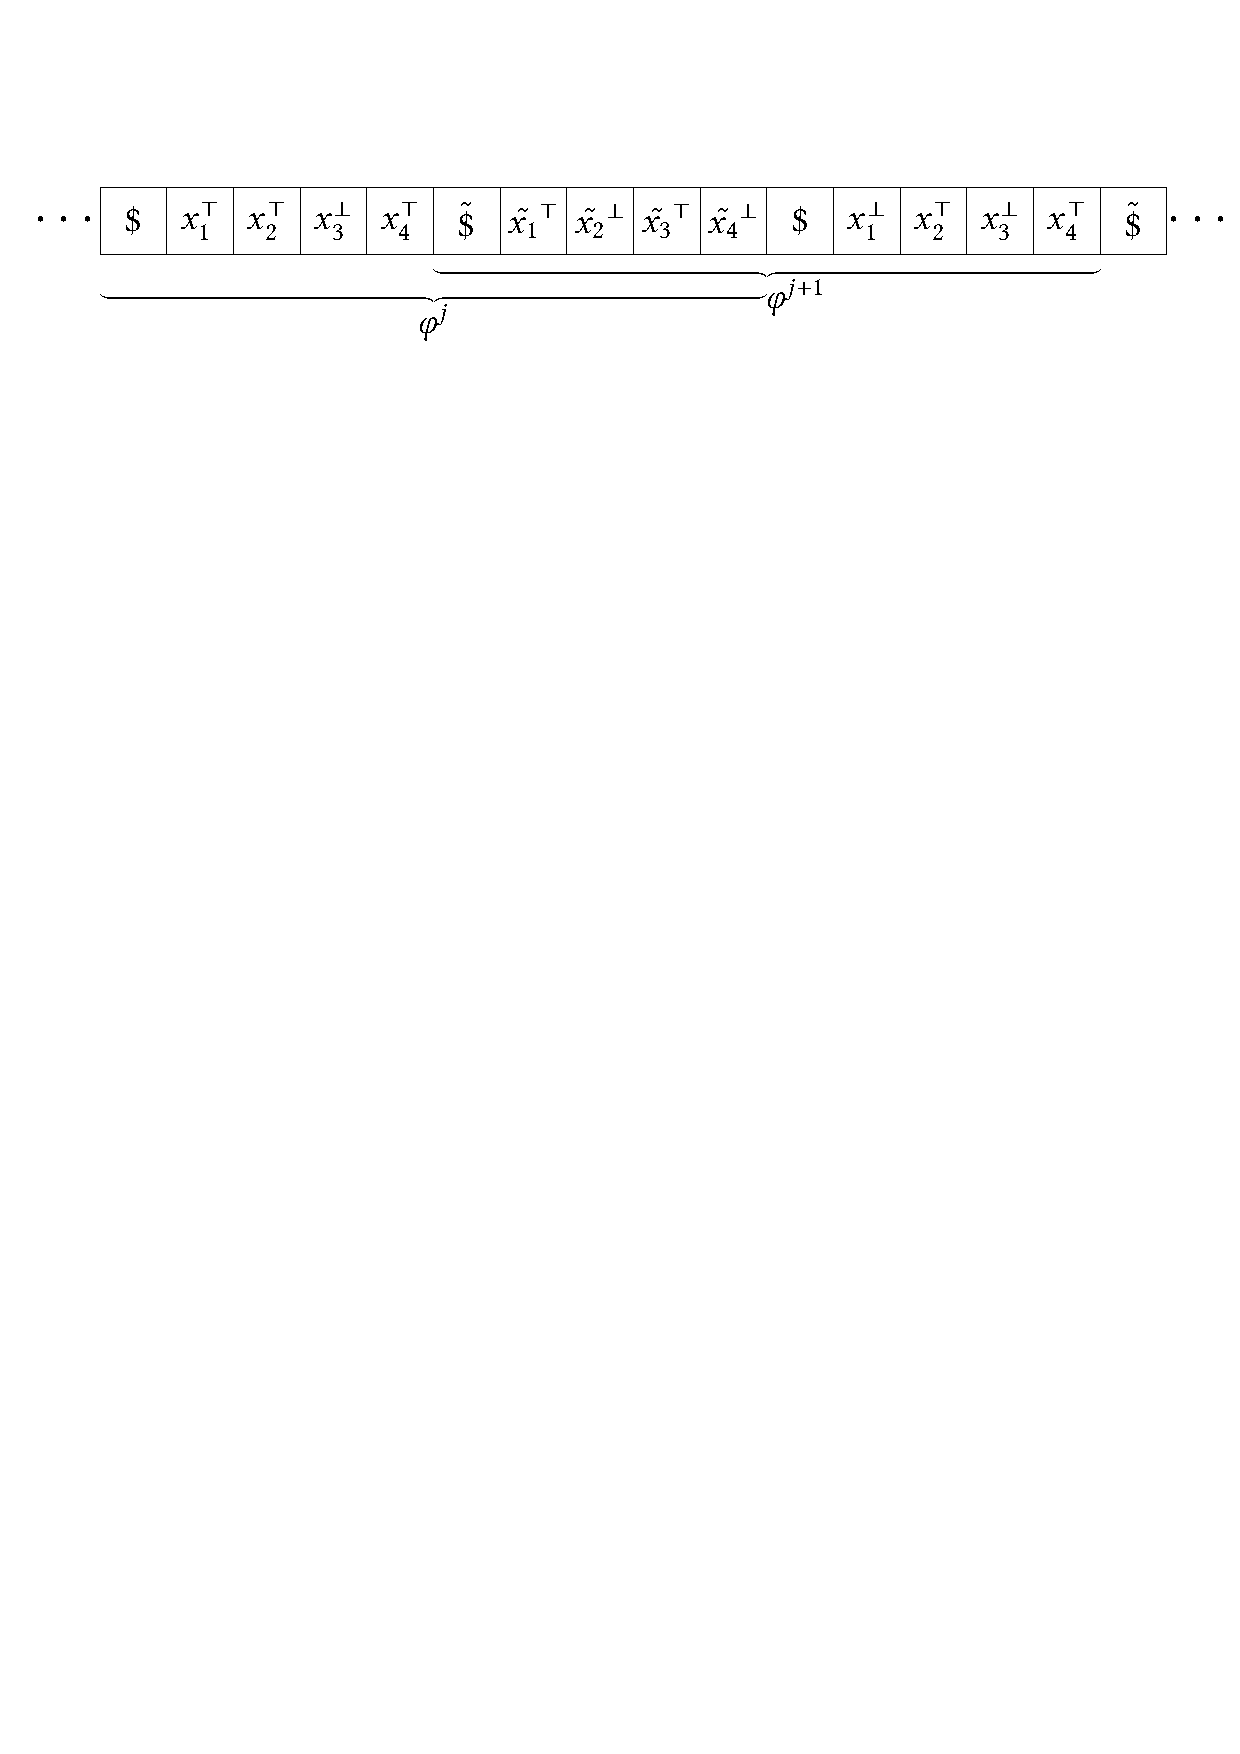
\includegraphics[width=\textwidth]{Chaps/Timelines/Psp.pdf}
    \caption{Let
    the formula $\varphi$ be defined over two sets of variables, $\Gamma=\{x_1,x_2,x_3,x_4\}$ and $\Gamma^{+1}=\{x_1^{+1},x_2^{+1},x_3^{+1},x_4^{+1}\}$. 
    The $j$-th copy (we assume $j$ is odd) of $\varphi$, i.e., $\varphi^j$, is satisfied by the assignment $x_1^j\mapsto \top$, $x_2^j\mapsto \top$, $x_3^j\mapsto \bot$, $x_4^j\mapsto \top$, $x_1^{j+1}\mapsto \top$, $x_2^{j+1}\mapsto \bot$, $x_3^{j+1}\mapsto \top$, $x_4^{j+1}\mapsto \bot$. The analogous for $\varphi^{j+1}$. }
    \label{fig:phij}
\end{figure}

We start with the next simple trigger rules, one for each $v\in V$: 
\[o[y=v]\to o\leq^{\mathsf{s},\mathsf{e}}_{[0,2]} o.\]
Paired with the constraint function $D$, they enforce
all tokens' durations to be \emph{exactly} 2: intuitively, since we exclude singular intervals, requiring, for instance, that a token $o'$ starts  $t$ instants of time after the end of $o$, with $t\in [\ell,\ell+1]$ and even $\ell\in\Nat$, boils down to $o'$ starting \emph{exactly} $\ell$ instants after the end of $o$. We also observe that, given the constant token duration, the density of the time domain does not play any role in this proof.

We now add the next rules:
\begin{itemize}
\item
    $\true \to \exists o[y=\$]. o\geq^{\mathsf{s}}_{[0,1]} 0$;
\item
    $\true \to \exists o[y=\tilde{\$}]. o\geq^{\mathsf{s}}_{[0,1]} (2^{2n}+1)\cdot 2(n+1)$;
\item
    $\true \to \exists o[y=stop]. o\geq^{\mathsf{s}}_{[0,1]} (2^{2n}+2)\cdot 2(n+1)$.
\end{itemize}
They respectively impose that $(i)$~a token with value $\$$ starts exactly at $t=0$ (recall that the duration of every token is 2);
$(ii)$~there exists a token with value $\tilde{\$}$ starting at $t=(2^{2n}+1)\cdot 2(n+1)$; 
$(iii)$~a token with value $stop$ starts at $t=(2^{2n}+2)\cdot 2(n+1)$. 
We are forcing the timeline to encode truth assignments for variables $x_1^1,\ldots, x_n^1,\ldots, x_1^{2^{2n}+2} ,\ldots , x_n^{2^{2n}+2}$: as a matter of fact, we will decide satisfiability of the finite formula $\Phi_f= \bigwedge_{j= 1}^{2^{2n}+1} \varphi^j$, which is equivalent to $\Phi$.

% The following rules require that, after a token with value $\$$ (resp., $\tilde{\$}$), there is a token with value $\tilde{\$}$ (resp., $\$$) or $stop$, after exactly $2n$ instants of time (recall that the transition function forces the presence of a token for each $x_i^j$ between near occurrences of $\$$/$\tilde{\$}$). 
% \[
%     a[y=\$]\to (\exists b[y=\tilde{\$}]. a\leq ^{\mathsf{e},\mathsf{s}}_{[0,2n]} b) \vee (\exists b[y=stop]. a\leq ^{\mathsf{e},\mathsf{s}}_{[0,2n]} b).
% \]
% \[
%     a[y=\tilde{\$}]\to (\exists b[y=\$]. a\leq ^{\mathsf{e},\mathsf{s}}_{[0,2n]} b) \vee (\exists b[y=stop]. a\leq ^{\mathsf{e},\mathsf{s}}_{[0,2n]} b).
% \]

We now consider the next rules, that enforce the satisfaction of each $\varphi^j$ or,
equivalently, of $\varphi$ over the assignments of $(x_1^j,\ldots, x_n^j, x_1^{j+1},\ldots, x_n^{j+1})$.

For the $t$-th conjunct of $\varphi$, % $1\leq t\leq m$, 
we define the future simple rule:
\begin{multline*}
    o[y=\tilde{\$}]\to \\
    \Big(\smashoperator{\bigvee_{x_i\in \Gamma\cap L^+_t}} \exists o'[y=\tilde{x_i}^\top]. o\leq ^{\mathsf{e},\mathsf{s}}_{[0,4n]} o' \Big) \vee 
        \Big(\smashoperator{\bigvee_{x_i^{+1}\in \Gamma^{+1}\cap L^+_t}} \exists o'[y=x_i^\top]. o\leq ^{\mathsf{e},\mathsf{s}}_{[0,4n]} o' \Big) \vee \\
        \Big(\smashoperator{\bigvee_{x_i\in \Gamma\cap L^-_t}} \exists o'[y=\tilde{x_i}^\bot]. o\leq ^{\mathsf{e},\mathsf{s}}_{[0,4n]} o' \Big) \vee 
        \Big(\smashoperator{\bigvee_{x_i^{+1}\in \Gamma^{+1}\cap L^-_t}} \exists o'[y=x_i^\bot]. o\leq ^{\mathsf{e},\mathsf{s}}_{[0,4n]} o' \Big) \vee \\
        \exists o''[y=stop]. o\leq ^{\mathsf{e},\mathsf{s}}_{[0,2n]} o''.
\end{multline*}
Basically, this rule (the rule where the trigger has value $\$$ being analogous) states that, after every occurrence of $\tilde{\$}$, a token $o'$, making true at least a (positive or negative) literal in the conjunct, must occur by $4n$ time instants (i.e., before the following occurrence of $\tilde{\$}$).
The disjunct $\exists o''[y=stop]. o\leq ^{\mathsf{e},\mathsf{s}}_{[0,2n]} o'' $ is present just to avoid evaluating $\varphi$ on the $n$ tokens before (the first occurrence of) $stop$.

%To conclude the proof we observe that the state variable 
The variable $y$ and all synchronization rules can be generated in time polynomial in $|\varphi|$ (in particular, all interval bounds and time constants of time-point atoms have a value, encoded in binary, in $O(2^{2n})$).
\end{proof}

By Theorem~\ref{theorem:UpperBounds} and Theorem~\ref{theorem:PSPlowerBound}, $\Psp$-completeness of 
future TP with simple trigger rules and intervals in $\Intv_{(0,\infty)}$ follows.

In the next section we focus on a different restriction of the TP problem, which will allow us to devise a $\NP$ planning algorithm for it.
\section{TP with trigger-less rules only is \NP-complete}\label{sec:NPtriggerless}

In this section we describe a TP algorithm,
for planning domains where only trigger-less rules are allowed,
which requires a polynomial number of (non-deterministic) computation steps.
We recall that trigger-less rules are useful, for instance, to express initial, intermediate conditions and reachability goals.

We want to start with the following example, with which we highlight that there is no \emph{polynomial-size} plan for some problem instances/domains. Thus, an explicit enumeration of all tokens of a multi-timeline \emph{does not} represent a suitable polynomial-size certificate.

\begin{example}
Let us consider the following planning domain.
We denote by $p(i)$ the $i$-th prime number, assuming $p(1)=1$, $p(2)=2$, $p(3)=3$, $p(4)=5$,\dots .
We define, for $i=1,\ldots,n$, the state variables $x_i=(\{v_i\},\{(v_i,v_i)\},D_{x_i})$ with $D_{x_i}(v_i)=\mathopen[p(i),p(i)\mathclose]$.
The following rule
\[
\true\to \exists o_1[x_1=v_1] \cdots \exists o_n[x_n=v_n].\bigwedge_{i=1}^{n-1} o_i\leq_{[0,0]}^{\mathsf{e},\mathsf{e}} o_{i+1}
\]
is asking for the existence of a \lq\lq synchronization point\rq\rq , where $n$ tokens (one for each variable) have their ends aligned.
Due to the allowed token durations, the first such time point is $\prod_{i=1}^{n} p(i)\geq 2^{n-1}$.
Hence, in any plan, the timeline for $x_1$ features at least $2^{n-1}$ tokens: no explicit polynomial-time enumeration of such tokens is possible.
\end{example}
%
As a consequence, there exists no trivial guess-and-check \NP\ algorithm.
Conversely, one can easily prove the following result.
\begin{theorem}
The TP problem with trigger-less rules only is \NP-hard, even with one state variable (under polynomial-time reductions).
\end{theorem}
\begin{proof}
There is a trivial reduction from the problem of the existence of a Hamiltonian path in a directed graph.

Given a directed graph $G=(V,E)$, with $|V|=n$, 
we define the state variable $x=(V,E,D_x)$, where $D_x(v)=[1,1]$ for each $v\in V$.
We add the following trigger-less rules, one for each $v\in V$:
\[
\true \to \exists o[x=v]. o\geq ^{\mathsf s}_{[0,n-1]} 0 .
\]
The rule for $v\in V$ requires that there is a token $(x,v,1)$ along the timeline for $x$, which starts no later than $n-1$.
It is easy to check that $G$ contains a Hamiltonian path if and only if there exists a plan for the defined planning domain.
\end{proof}

We now present the aforementioned non-deterministic polynomial-time algorithm, proving that timeline-based planning with trigger-less rules is in \NP.

We preliminarily have to derive a \emph{finite horizon} (namely, the end time of the last token) for the plans of a (any) instance of TP with trigger-less rules. That is, 
if an instance $P=(SV,R)$ admits a plan, then $P$ also has a plan whose horizon is no greater than a given bound. Analogously, we have to calculate a \emph{bound to the maximum number of tokens} in a plan.
Both can be obtained from 
the constructions of the \TA s described in the proof of 
Theorem~\ref{theorem:UpperBounds}:
since only trigger-less rules are now allowed,
we disregard the construction of the \MTL\ formula $\varphi_\forall$,
and restrict our attention to the \TA\  
$\Au_P$ (i.e., the intersection between $\Au_{SV}$ for the state variables in $SV$ from Proposition~\ref{prop:AtutomataForMultiTimeline} and $\Au_{_\exists}$ for the trigger-less rules in $R$ from Proposition~\ref{prop:TATriggerLessRules}), which has $\alpha_s=2^{O(N_q+\sum_{x\in SV} |V_x|)}$ states, $\alpha_c=O(N_q+|SV|)$ clocks and maximum constant $\alpha_K=O(K_p)$, where
$N_q$  is the overall number of quantifiers   in the trigger-less  rules of $R$, 
and accepts all and only the encodings $w_\Pi$ of multi-timelines $\Pi$ of $SV$ satisfying all the trigger-less rules in $R$.

The language emptiness checking algorithm for \TA s executed over $\Au_P$ visits the (untimed) region automaton for $\Au_P$~\cite{ALUR1994183},
which features $\alpha=\alpha_s\cdot O(\alpha_c!\cdot 2^{\alpha_c}\cdot 2^{2 N_q^2}\cdot (2\alpha_K +2)^{\alpha_c})$
states%
\footnote{The factor $2^{2 N_q^2}$ is present due to diagonal clock constraints in $\Au_P$.}%
, trying to find a path, from the initial state to a final state, whose length can clearly be bounded by the number of states.
%
We observe that each edge/transition of the region automaton in such a path corresponds, in the worst case, to the start point of a token for each timeline for the variables in $SV$ (i.e., assuming that all these tokens start simultaneously).
This yields a bound on the number of tokens, which is $\alpha \cdot |SV|$.
We can also derive a bound on the horizon of the plan, which is $\alpha \cdot |SV| \cdot (\alpha_K+1)$, as every transition taken in $\Au_P$ may let at most $\alpha_K+1$ time units pass, as $\alpha_K$ accounts in particular for the maximum constant to which a (any) clock is compared.\footnote{Clearly, and unbounded quantity of time units may pass, but after $\alpha_K+1$ the last region of the region automaton will certainly have been reached.}

Having this pair of bounds, 
we are now ready to describe the two main phases of the algorithm, corresponding to the following pair of observations.
On the one hand, $(i)$~each trigger-less rule requires, as we said,
the existence of an \emph{a priori bounded number} of temporal events satisfying mutual temporal relations (namely, in the worst case, the start time and end time of all tokens associated with the quantifiers of one of its existential statements).
On the other hand, $(ii)$~timelines for different state variables evolve independently of each other.
In order to deal with $(i)$, we non-deterministically position such temporal events along timelines; as for $(ii)$, we enforce a correct evolution of each timeline between pairs of \lq\lq positioned\rq\rq\ events, completely independently of the other timelines.

% \paragraph{Preprocessing}
% As a preliminary preprocessing phase, we consider all rational values occurring in the input planning problem $P=(SV,S)$---be either 
% upper/lower bounds of an interval of a token duration, a time constant in an atom, or 
% upper/lower bounds ($u$ or $\ell$) at the subscript of an atom---and make them integers by multiplying them
% by the least common multiple $\gamma$ of all denominators. This involves a quadratic blowup in the input size, being all constants encoded in binary. 

% It is routine to check that, having a plan for $P'$---where all values are integers---we can obtain one for the original $P$, by dividing the start/end times of all tokens in each timeline by $\gamma$.

\paragraph{Non-deterministic token positioning.}
The algorithm starts by non-determin\-istically selecting, for every trigger-less rule in $R$, a disjunct---and deleting all the others. Then, for every (left) quantifier $o_i[x_i=v_i]$, it generates the integer part of both the start and the end time of the token for $x_i$ to which $o_i$ is mapped. We call such time instants, respectively, $\mathsf{s}_{int}(o_i)$ and $\mathsf{e}_{int}(o_i)$.\footnote{We can assume w.l.o.g.\ that all quantifiers refer to distinct tokens. As a matter of fact, the algorithm can non-deterministically choose to make two (or more) quantifiers $o_i[x_i=v_i]$ and $o_j[x_i=v_i]$ over the same variable and value \lq\lq collapse\rq\rq\ to the same token just by rewriting all occurrences of $o_j$ as $o_i$ in the atoms of the rules.} We observe that all start/end time $\mathsf{s}_{int}(o_i)$ and $\mathsf{e}_{int}(o_i)$, being less or equal to $\alpha \cdot |SV| \cdot (\alpha_K+1)$ (the finite horizon bound), have an integer part that can be encoded with polynomially many bits (and thus can be generated in polynomial time). 
%Let $\xi$ denote the number of quantifiers of all rules. 

Let us now consider the fractional parts of the start/end time of the tokens associated with quantifiers. We denote them by $\mathsf{s}_{frac}(o_i)$ and $\mathsf{e}_{frac}(o_i)$. The algorithm non-deterministically generates an \emph{order} of all such fractional parts. In particular we have to specify, for every token start/end time, whether it is integer ($\mathsf{s}_{frac}(o_i)=0$, $\mathsf{e}_{frac}(o_i)=0$) or not ($\mathsf{s}_{frac}(o_i)>0$, $\mathsf{e}_{frac}(o_i)>0$).
%There are $2^{2\xi}\cdot 2^{2\xi}\cdot (2\xi)!$ such possibilities, and each one can be encoded in binary.
Every such possibility can be generated in polynomial time.

Some trivial tests should now be performed, namely that, for all $o_i$, $\mathsf{s}_{int}(o_i)\leq \mathsf{e}_{int}(o_i)$, each token is assigned an end time equal or greater than its start time, and no two tokens for the same variable are overlapping.

It is routine to check that, if we change the start/end time of (some of the) tokens associated with quantifiers, 
but we leave unchanged $(i)$~all the integer parts, $(ii)$~zeroness/non-zeroness of fractional parts, and $(iii)$~the fractional parts' order,
then the satisfaction of the (atoms in the) trigger-less rules does not change. This is due to all the constants being integers.%
%, as a result of the preprocessing step.
\footnote{We may observe that, by leaving unchanged all the integer parts and the fractional parts' order, the region of the region graph of the timed automaton does not change.} Therefore we can now check whether all rules are satisfied.

\paragraph{Enforcing legal token durations and timeline evolutions.}

We now continue by checking that: $(i)$ all tokens associated with a quantifier have a legal duration, and that $(ii)$ there exists a legal timeline evolution between pairs of adjacent such tokens over the same variable (here \emph{adjacent} means that there is no other token associated with a quantifier in between). 
We will enforce all these requirements as constraints of a \emph{linear problem}, which can be solved in deterministic polynomial time (e.g., using the ellipsoid algorithm).
When needed, we use \emph{strict inequalities}, which are not allowed in linear programs. We shall show later how to convert these into non-strict ones.

We start by associating non-negative variables $\alpha_{o_i,s}, \alpha_{o_i,e}$ with the fractional parts of the start/end times $\mathsf{s}_{frac}(o_i)$, $\mathsf{e}_{frac}(o_i)$ of every token for a quantifier $o_i[x_i=v_i]$.
First, we add the linear constraints
\begin{equation*}
    0\leq \alpha_{o_i,s}<1,\quad 0\leq \alpha_{o_i,e}<1.
\end{equation*}
Then, we also need to enforce that the values of $\alpha_{o_i,s}, \alpha_{o_i,e}$ respect the decided order of the fractional parts: for example,
\begin{equation*}
    0=\alpha_{o_i,s}=\alpha_{o_j,s}<\alpha_{o_k,s}<\ldots <\alpha_{o_j,e}<\alpha_{o_i,e}=\alpha_{o_k,e}<\ldots
\end{equation*}
%
To enforce requirement $(i)$, we set, for all $o_i[x_i=v_i]$,
\begin{equation*}
    a\leq (\mathsf{e}_{int}(o_i)+\alpha_{o_i,e})-(\mathsf{s}_{int}(o_i)+\alpha_{o_i,s})\leq b
\end{equation*}
where $D_{x_i}(v_i)=\mathopen[a,b\mathclose]$. Clearly, strict ($<$) inequalities must be used for a left/right open interval.

To enforce requirement $(ii)$, namely that there exists a legal timeline evolution between each pair of adjacent tokens for the same state variable, say $o_i[x_i=v_i]$ and $o_j[x_i=v_j]$, we proceed as follows (for a correct evolution between $t=0$ and the first token, analogous considerations can be made).

Let us consider each state variable $x_i=(V_i,T_i,D_i)$ as a directed graph $G=(V_i,T_i)$ where 
$D_i$ is a function associating with each vertex $v\in V_i$ a duration range.
We have to decide whether or not there exist
\begin{itemize}
    \item a path in $G$, possibly with repeated vertices and edges, $v_0 \cdot v_1 \cdots v_{n-1}\cdot v_n$, where $v_0\in T_i(v_i)$ and $v_n$ with $v_j\in T_i(v_n)$ are non-deterministically generated, and
    \item a list of non-negative real values $d_0,\ldots,d_n$,
such that 
\[\sum_{t=0}^n d_t = (\mathsf{s}_{int}(o_j)+\alpha_{o_j,s}) - (\mathsf{e}_{int}(o_i)+\alpha_{o_i,e}),\]
and for all $s=0,\ldots, n$, $d_s\in D_i(v_s)$.
\end{itemize}
%  -  
%  - 

% Intuitively, we have to find a path in $G$, possibly where we get to the same vertices/edges also more than once, and where we remain in each vertex a non-negative rational amount of time allowed by the minimum/maximum duration function, such that the overall time of the path equals $h$.

We guess 
a set of integers $\{\alpha'_{u,v}\mid (u,v)\in T_i\}$.
Intuitively, $\alpha'_{u,v}$ is the number of times the solution path
traverses $(u,v)$. Since every time an edge is traversed a new token starts, each $\alpha'_{u,v}$ is bounded by the number of tokens, i.e., by $\alpha \cdot |SV|$. Hence the binary encoding of $\alpha'_{u,v}$ can be generated in polynomial time.

We then perform the following deterministic steps.
\begin{enumerate}
\item We consider the subset $E'$ of edges of $G$, $E'=\{(u,v)\in T_i\mid \alpha'_{u,v}>0\}$. We check whether $E'$ induces a strongly (undirected) connected subgraph of $G$.
\item We check whether 
    \begin{itemize}
        \item $\sum_{(u,v)\in E'} \alpha'_{u,v}=\sum_{(v,w)\in E'} \alpha'_{v,w}$, for all $v \in V_i\setminus\{v_0,v_n\}$;
        \item $\sum_{(u,v_0)\in E'} \alpha'_{u,v_0}=\sum_{(v_0,w)\in E'} \alpha'_{v_0,w}-1$;
        \item $\sum_{(u,v_n)\in E'} \alpha'_{u,v_n}=\sum_{(v_n,w)\in E'} \alpha'_{v_n,w}+1$.
    \end{itemize}

\item For all $v \in V_i\setminus\{v_0\}$, we define $y_v=\sum_{(u,v)\in E'} \alpha'_{u,v}$ ($y_v$ is the number of times the solution path gets into $v$). Moreover, 
$y_{v_0} = \sum_{(v_0,u)\in E'} \alpha'_{v_0,u}$.
\item We define the real non-negative variables $z_v$, for every $v \in V_i$ ($z_v$ is the total waiting time of the path on the node $v$), subject to the following constraints:
\[a\cdot y_v \leq z_v \leq b\cdot y_v,\]
where $D_i(v)=[a,b]$ (an analogous constraint should be written for open intervals). Finally we set:
\[\sum_{v \in V_i} z_v = (\mathsf{s}_{int}(o_j)+\alpha_{o_j,s}) - (\mathsf{e}_{int}(o_i)+\alpha_{o_i,e}).\]
\end{enumerate}

Steps (1.) and (2.) together check that the values $\alpha'_{u,v}$ for the arcs specify
a directed Eulerian path from $v_0$ to $v_n$ in a multigraph. Indeed,
the following theorem holds.
\begin{theorem}\cite{Jung}
Let $G'=(V',E')$ be a directed multigraph ($E'$ is a multiset).
$G'$ has a (directed) Eulerian path from $v_0$ to $v_n$ if and only if:
\begin{itemize}
    \item the undirected version of $G'$ is connected, and
    \item $|\{(u,v)\in E'\}| =| \{(v,w)\in E'\}|$, for all $v \in V'\setminus\{v_0,v_n\}$;
    \item $|\{(u,v_0)\in E'\}|=|\{(v_0,w)\in E'\}|-1$;
    \item $|\{(u,v_n)\in E'\}|=|\{(v_n,w)\in E'\}|+1$.
\end{itemize}
\end{theorem}

Steps (3.) and (4.) evaluate the waiting times of the path in some
vertex $v$ with duration interval $\mathopen[a,b\mathclose]$.
If the solution path visits the vertex $y_v$ times, then every single
visit must take at least $a$ and at most $b$ units of time.
Hence the overall visitation time is in between $a\cdot y_v$ and
$b\cdot y_v$.
Vice versa, if the total visitation time is in between $a\cdot y_v$ and
 $b\cdot y_v$, then it can be slit into $y_v$ intervals, each one falling into $\mathopen[a,b\mathclose]$. 

The algorithm concludes by solving the linear program given by the variables $\alpha_{o_i,s}$ and $\alpha_{o_i,e}$ for each quantifier $o_i[x_i=v_i]$, and for each pair of adjacent tokens in the same timeline for $x_i$, for each $v\in V_i$, the variables $z_v$ subject to their constraints.

Finally, in order to conform to linear programming, we have to replace all strict inequalities with non-strict ones.
It is straightforward to observe that all constraints involving strict inequalities we have written so far are of
(or can easily be converted into) the following forms: 
$\xi s<\eta q+k$ or $\xi s>\eta q+k$, where $s$ and $q$ are variables, and $\xi$, $\eta$, $k$ are constants.
We replace them, respectively, by $\xi s-\eta q-k+\beta_t\leq 0$ and $\xi s-\eta q-k-\beta_t\geq 0$, where $\beta_t$ is an additional fresh non-negative variable, which is \emph{local} to a single constraint. 
We observe that the original inequality and the new one are equivalent if and only if $\beta_t$ is a small enough \emph{positive} number.
Moreover, we add another non-negative variable, say $r$, which is subject to a constraint $r\leq \beta_t$, for each of the introduced variables $\beta_t$ (i.e., $r$ is less than or equal to the minimum of all $\beta_t$'s). Finally, we maximize the value of $r$ when solving the linear program. We have that $\max r>0$ if and only if there is an admissible solution where the values of all $\beta_t$'s are positive (and thus the original strict inequalities hold true). 

This ends the description of the planning algorithm. We can thus conclude the section with the main result.
\begin{theorem}
The TP problem with trigger-less rules only is \NP-complete.
\end{theorem}

In the next section, using the results on the variants of the TP problem, we shall study MC over timelines.
\section{MC for \MITL\ over timelines}\label{sec:modelcheckingTimelines}

In this section we deal with the ultimate goal of the present chapter:
as mentioned, we want to model check systems specified in terms of timelines. More precisely, 
a system is described as a set of state variables along with a set of synchronization rules over them (a TP domain) $P=(SV,R)$.
As mentioned in the introduction, the property specification language we will be assuming is the logic \MITL.
%%
%Henceforth, $\Prop$ denotes a set of proposition letters.

We first recall the encoding of multi-timelines already adopted in Section~\ref{sec:Reduction}, 
over which we interpret \MITL,
that exploits 
the set $\Prop$ of proposition letters
\[
\Prop = \bigcup_{x\in SV}\Main_x \cup \Deriv ,
\] 
where in particular
\[
\Main_x = ((\{\Beg_x \}\cup V_x) \times V_x)   \cup   (V_x \times \{\End_x\}).
\]
The tags $\Beg_x$ and $\End_x$ mark the beginning and the end of a timeline for $x$, and a pair $(v,v')\in \Main_x$ represents a 
transition of the value taken by $x$ from $v$ to $v'$ (a token for $x$ with value $v'$ follows a token with value $v$).
The already introduced formula 
\[
\psi(\start,v)= (\Beg_x,v)\vee \displaystyle{\bigvee_{u\in V_x}}(u,v),
\]
states that a start-event for a token for $x$ with value $v$ occurs at the current time.
Finally, $\EqTime(\theta) = \theta \vee [\neg p_> \StrictUntil_{\geq 0}(\neg p_> \wedge \theta)]$, where $p_>\in\Deriv$, is satisfied
by an encoding of a multi-timeline at the current time if $\theta$ eventually holds at a position whose timestamp coincides with the current one.

Before formalizing the \emph{MC problem for \MITL\ formulas over timelines}, we want to start with an easy example of a system whose components are described by timelines, over which we check some properties encoded by \MITL\ formulas.

\begin{figure}[p]
    \centering
    \resizebox{!}{0.9\textheight}{\rotatebox{90}{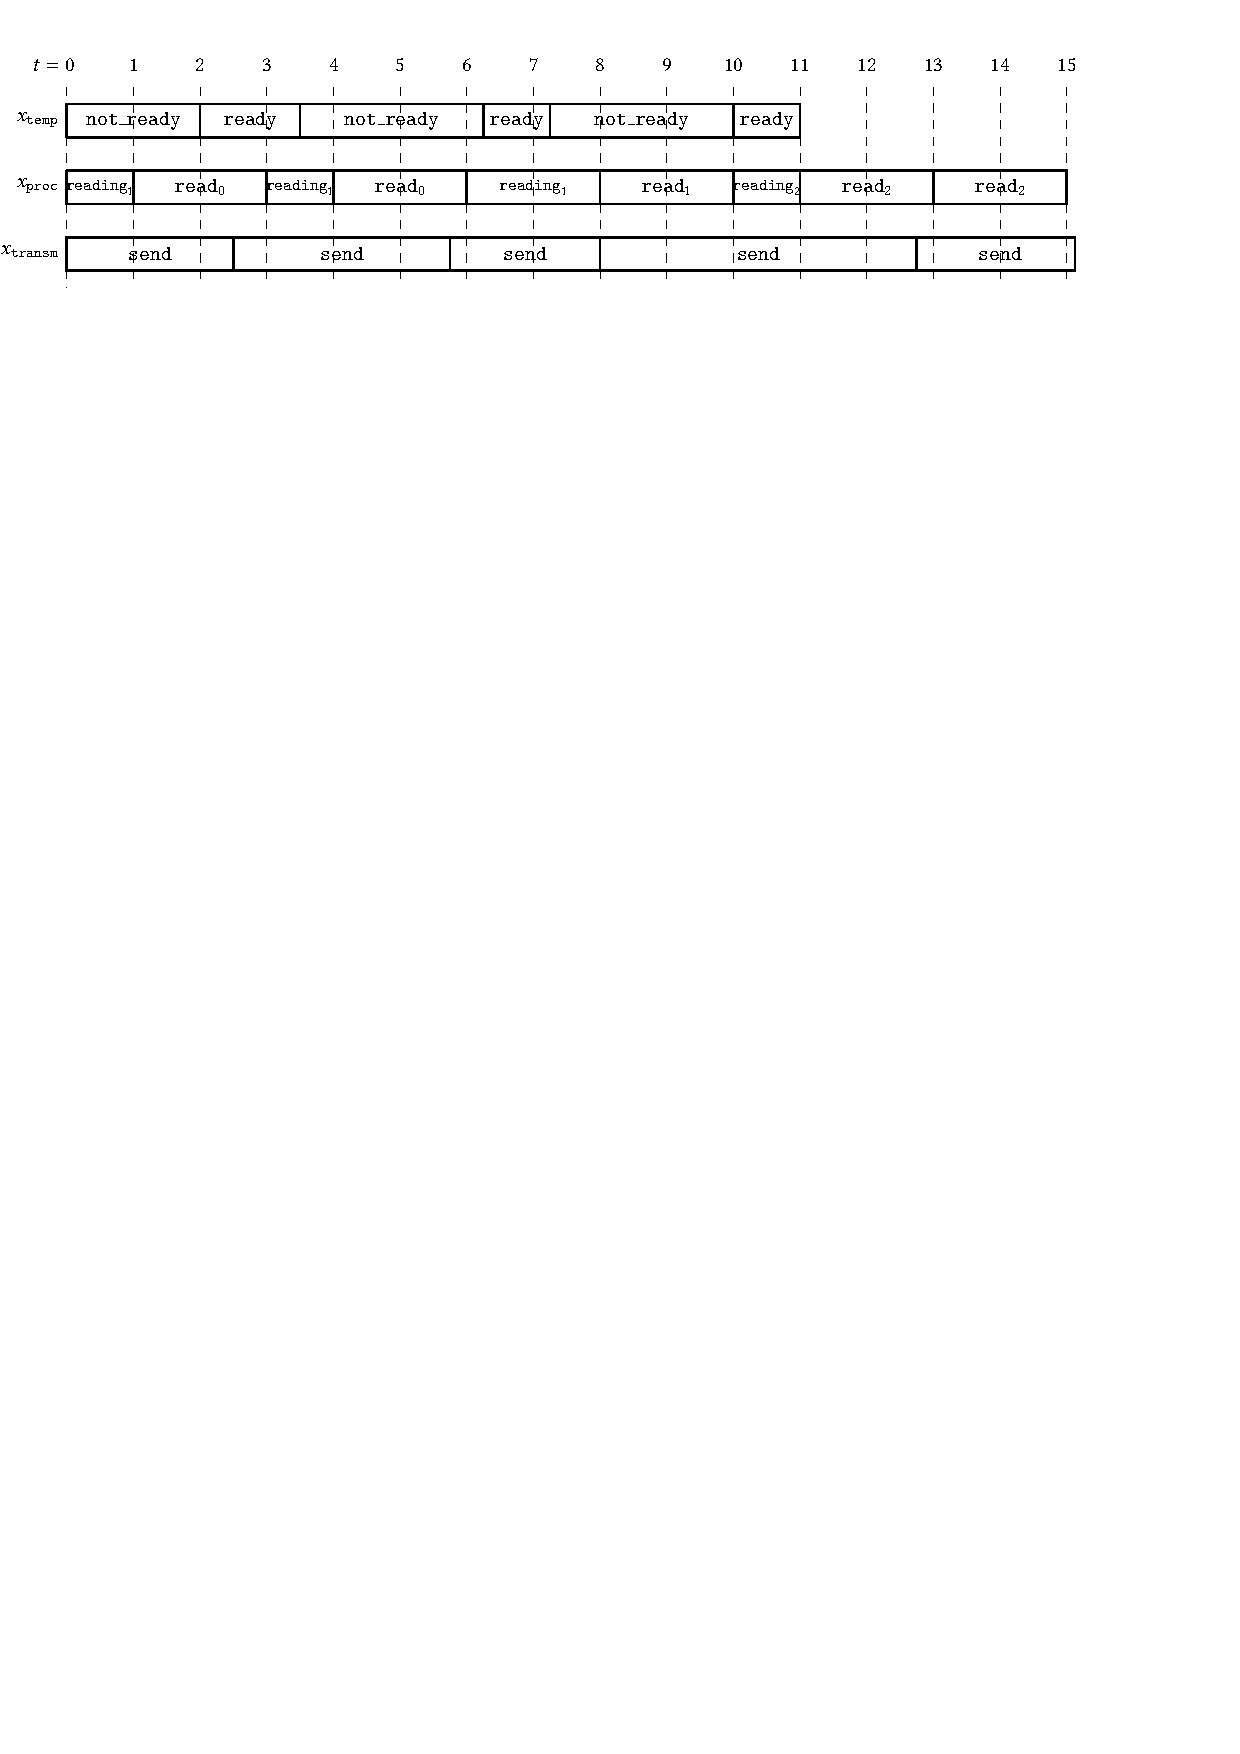
\includegraphics{Chaps/Timelines/exPlan.pdf}}}
    \caption{Example of computation for the defined system}
    \label{fig:explan}
\end{figure}

\begin{example}
Let us consider the following system, consisting of a \emph{temperature sensor}, a \emph{processing unit}, and a \emph{data transmission unit}.
These components are modelled by three state variables, $x_\mathtt{temp}=(V_\mathtt{temp},T_\mathtt{temp},D_\mathtt{temp})$, $x_\mathtt{proc}=(V_\mathtt{proc},T_\mathtt{proc},D_\mathtt{proc})$ and $x_\mathtt{transm}=(V_\mathtt{transm},T_\mathtt{transm},D_\mathtt{transm})$, where
\begin{itemize}
    \item $V_\mathtt{temp}=\{\mathtt{ready}, \mathtt{not\_ready}\}$, \\
    $T_\mathtt{temp}(\mathtt{ready})=\{\mathtt{not\_ready}\}$, $T_\mathtt{temp}(\mathtt{not\_ready})=\{\mathtt{ready}\}$, \\ $D_\mathtt{temp}(\mathtt{ready})=[1,2]$, $D_\mathtt{temp}(\mathtt{not\_ready})=[2,3]$;
    \item $V_\mathtt{proc}=\{\mathtt{reading}_1,\mathtt{reading}_2,\mathtt{read}_0,\mathtt{read}_1,\mathtt{read}_2\}$, \\
    $T_\mathtt{proc}(\mathtt{reading}_1)=\{\mathtt{read}_0,\mathtt{read}_1\}$,
    $T_\mathtt{proc}(\mathtt{reading}_2)=\{\mathtt{read}_1,\allowbreak \mathtt{read}_2\}$,
    $T_\mathtt{proc}(\mathtt{read}_0)=\{\mathtt{reading}_1\}$, $T_\mathtt{proc}(\mathtt{read}_1)=\{\mathtt{reading}_2\}$,
    $T_\mathtt{proc}(\mathtt{read}_2)=\{\mathtt{read}_2\}$, \\
    $D_\mathtt{proc}(\mathtt{reading}_1)=D_\mathtt{proc}(\mathtt{reading}_2)=[1,2]$, $D_\mathtt{proc}(\mathtt{read}_0)=D_\mathtt{proc}(\mathtt{read}_1)=D_\mathtt{proc}(\mathtt{read}_2)=[2,3]$;
    \item $V_\mathtt{transm}=\{\mathtt{send}\}$,\\
    $T_\mathtt{transm}(\mathtt{send})=\{\mathtt{send}\}$,\\
    $D_\mathtt{transm}(\mathtt{send})=[2,5]$.
\end{itemize}

The temperature sensor alternates between the two states $\mathtt{ready}$ and $\mathtt{not\_ready}$. In the former, it senses the temperature of the environment and \emph{possibly} sends the temperature value to the processing unit.
The purpose of the processing unit is receiving \emph{two} temperature samples from the sensor, and sending the average value to the data transmission unit. While in state $\mathtt{read}_i$, for $i=0,1,2$, it has read $i$ samples. While in $\mathtt{reading}_j$, for $j=1,2$, it is attempting to read the $j$-th sample. A reading is possible only if the sensor and the processing unit are synchronized: a time interval (token) with value $\mathtt{reading}_j$ has to \emph{contain} (Allen relation, see Table~\ref{allen}) a token $\mathtt{ready}$. 
Analogously, the processing unit can send data to the transmitter only if a token with value $\mathtt{send}$ contains one with value $\mathtt{read}_2$.

The sensor starts in state $\mathtt{not\_ready}$. This is specified by the trigger-less rule $\true\to\exists o[x_\mathtt{temp} = \mathtt{not\_ready}]. o\leq^\start_{[0,0]} 0$. The processing unit starts in state $\mathtt{reading}_1$: $\true\to\exists o[x_\mathtt{proc} = \mathtt{reading}_1]. o\leq^\start_{[0,0]} 0$.
(Recall that trigger-less rules may also contain singular intervals at no extra computational cost.)
The goal of the system is encoded by the rule
$\true\to \exists o_1 [x_\mathtt{proc} = \mathtt{read}_2] \exists o_2 [x_\mathtt{transm} = \mathtt{send}]. (o_2 \leq^{\start,\start}_{\mathopen[0,+\infty\mathclose[} o_1 \wedge o_1 \leq^{\Ending,\Ending}_{\mathopen[0,+\infty\mathclose[} o_2)$.

Let us now encode the fact that the sensor and the processing unit must be synchronized for the latter to receive a temperature sample.
We assume the next simple trigger rule to be \emph{interpreted under the future semantics}.
\begin{multline}\label{eq:sync}
o[x_\mathtt{proc} = \mathtt{reading}_1] \to (\exists o_1[x_\mathtt{proc} = \mathtt{read}_0]. o \leq_{[0,1]}^{\Ending,\start} o_1) \vee\\ (\exists o_2[x_\mathtt{proc} = \mathtt{read}_1] \exists o_3[x_\mathtt{temp} = \mathtt{ready}]. o \leq_{[0,1]}^{\Ending,\start} o_2\wedge o_3\leq_{\mathopen[0,+\infty\mathclose[}^{\Ending,\Ending} o).
\end{multline}
Let us observe that, due to the future semantics, the token (referenced by the name) $o$ starts no later than $o_3$: this with the interval atom \mbox{$o_3\leq_{\mathopen[0,+\infty\mathclose[}^{\Ending,\Ending} o$} force the \emph{contains} Allen relation between $o$ and $o_3$.
An analogous rule can be written for the second temperature sample (where $x_\mathtt{proc}=\mathtt{reading}_2$).

In Figure~\ref{fig:explan} we show an example of plan/computation for the system described by $P=(\{x_\mathtt{temp},x_\mathtt{proc},x_\mathtt{transm}\},R)$.

Let us now specify some properties in \MITL\ (more precisely, $\MITLR$) to check on the system model. The idea is that such properties must hold true over \emph{all possible computations (plans)} of the described system, in order for the MC problem to be satisfied.

\begin{itemize}
    \item $\Always_{<2}\;\neg \psi(\start,\mathtt{ready})$. This property holds true in any system computation, as the sensor does not ever get ready by 2 seconds;
    \item $\Eventually_{\leq 8}\; \psi(\start,\mathtt{read}_1)$. This property is not true in all computations (but it is, e.g., in the one of Figure~\ref{fig:explan}), because the sensor and the processing unit may synchronize for the first time after 8 seconds;
    \item $\Eventually_{\geq 0}\big(\psi(\start,\mathtt{ready}) \wedge (\true\until_{>0}\;\psi(\start,\mathtt{ready}))\big)$. This property holds true in any system computation, since the system guarantees, after some time, to eventually send the data via the transmitter. In order for this to happen, the sensor must become ready (at least) twice.
    \item $\Always_{\geq 0} \big(\psi(\start,\mathtt{read}_1) \to \Eventually_{\leq 3}\; \psi(\start,\mathtt{read}_2)\big)$. % \!\wedge\! (\EqTime(\psi(\start,\mathtt{send}))\!\vee\! \Past_\mathtt{send}^{\start}) \big)$. 
    This property is not true in all computations as the processing unit, after reading the first sample, may not be able to read the second one by 3 time units (e.g., when the transmitter and the processing unit do not synchronize as soon as possible).
    \item {\small $\Always_{\geq 0} \big(\psi(\start,\mathtt{reading}_1) \!\wedge\! (\EqTime(\psi(\start,\mathtt{ready}))\!\vee\! \Past_\mathtt{ready}^{\start}) \!\to\! \Eventually_{\leq 2}\, \psi(\start,\mathtt{read}_1) \big)$}. 
    We recall that the proposition letter $\Past_\mathtt{ready}^{\start}$ is true at the time it is interpreted if there is a past token for $x_\mathtt{temp}$ with value $\mathtt{ready}$ starting at the same timestamp. 
%
    The formula considers a situation where a token with value $\mathtt{reading}_1$ starts together with a token $\mathtt{ready}$. %Since the minum duration of is less than the minimum of, this is a synch. However,
    The property expressed by the formula is not true in general, as either 
    $(i)$~the token $\mathtt{reading}_1$ may not contain the token $\mathtt{ready}$, hence $x_\mathtt{proc}$ will not move to the state $\mathtt{read}_1$ by 2 time units, or
    $(ii)$~the token $\mathtt{reading}_1$ is followed by a token $\mathtt{read}_0$. As for the latter case,
    the system description rule (\ref{eq:sync}) states that if there is a transition from state $\mathtt{reading}_1$ to $\mathtt{read}_1$, then the processing unit and the sensors must have synchronized. However, the converse implication need not hold: the two component may fail to communicate anyway (the processing unit remaining in $\mathtt{read}_0$).
\end{itemize}
\end{example}

Let us now formally define the MC problem for \MITL\ formulas over timelines.
As shown in the proof of Theorem~\ref{theorem:UpperBounds}, given a system model $P_\text{sys}=(SV,R)$, it is possible to build a \TA\ $\mathcal{A}_\text{sys}$ that
accepts all and only the encodings $w_\Pi$ of multi-timelines $\Pi$ of $SV$ satisfying all the rules in $R$.

\begin{definition}[Model checking]
Given a system model $P_\text{sys}=(SV,R)$ and a \MITL\ formula $\varphi$ over $\Prop$, the MC problem for \MITL\ formulas over timelines is to decide whether or not $\TLang(\mathcal{A}_\text{sys})\subseteq \TLang(\varphi)$.
\end{definition}

We recall that~\cite{Alur:1996} %, as already mentioned in the proof of Theorem~\ref{theorem:UpperBounds}, 
given a \MITL\ (resp., $\MITLR$) formula $\psi$, where $N$ is the number of distinct subformulas of $\psi$, and $K$ the largest integer constant appearing in $\psi$, we can build a \TA\ $\mathcal{A}_\psi$ accepting the models of $\psi$, with $O(2^{N\cdot K})$ (resp., $O(2^{N})$) states, $O(N\cdot K)$ (resp., $O(N)$) clocks, and maximum constant $O(K)$. Deciding its emptiness requires
space \emph{logarithmic} in the number of states of $\mathcal{A}_\psi$ and \emph{polynomial}
in the number of clocks and in the length of the encoding of $K$, hence
exponential (resp., polynomial) space.

To decide if $\TLang(\mathcal{A}_\text{sys})\subseteq \TLang(\varphi)$, we check whether $\TLang(\mathcal{A}_\text{sys})\cap \TLang(\mathcal{A}_{\neg \varphi})= \emptyset$ by making the intersection $\mathcal{A}_\wedge$ of 
$\mathcal{A}_\text{sys}$ and $\mathcal{A}_{\neg \varphi}$, and checking for emptiness of its timed language. 
The size of $\mathcal{A}_\wedge$ is polynomial in those of $\mathcal{A}_\text{sys}$ and $ \mathcal{A}_{\neg \varphi}$.
Moreover $\mathcal{A}_\text{sys}$, $\mathcal{A}_{\neg \varphi}$ and $\mathcal{A}_\wedge$ can be built on the fly, and the emptiness test can be done without explicitly constructing them as well.
The next result follows by these observations and by Theorem~\ref{theorem:UpperBounds}.

\begin{theorem}
The MC problem for \MITL\ formulas over timelines, with simple future trigger rules and non-singular intervals, is in \EXPSPACE.

The MC problem for $\MITLR$ formulas over timelines, with simple future trigger rules and intervals in $\Intv_{(0,\infty)}$, is in \Psp.
\end{theorem}

Clearly, \EXPSPACE- and \Psp-completeness of the above MC problems follow by the underlying future TP problems.
% %%%%%%%%%%%%%%%%%%%%%%%%%%%%%%%%%%%%%%%%%%%%%%%%%%%%%%%%%%%%%%%%%%%%%%
% The Introduction:
% %%%%%%%%%%%%%%%%%%%%%%%%%%%%%%%%%%%%%%%%%%%%%%%%%%%%%%%%%%%%%%%%%%%%%%
\fancychapter{Conclusions and Future Work}
\label{cap:conclusions}

Conclusions Chapter

\cleardoublepage